% multiple1902 <multiple1902@gmail.com>
% bachelor.tex
% Copyright 2011~2012, multiple1902 (Weisi Dai)
% https://code.google.com/p/xjtuthesis/
% 
% It is strongly recommended that you read documentations located at
%   http://code.google.com/p/xjtuthesis/wiki/Landing?tm=6
% in advance of your compilation if you have not read them before.
%
% This work may be distributed and/or modified under the
% conditions of the LaTeX Project Public License, either version 1.3
% of this license or (at your option) any later version.
% The latest version of this license is in
%   http://www.latex-project.org/lppl.txt
% and version 1.3 or later is part of all distributions of LaTeX
% version 2005/12/01 or later.
%
% This work has the LPPL maintenance status `maintained'.
% 
% The Current Maintainer of this work is Weisi Dai.
%
\documentclass[
    bachelor, 
    %bigskip, % sets linespread factor to 1.5
    truefont, % just turn it on when using Windows
    %nofont, % remember to manally set the fonts
    pdflinks,
    %colorlinks,
    compact,
    ]{xjtuthesis}

% Compact is enabled so that blank page VI does not appear

\graphicspath{{figures/}}

\begin{document}
% multiple1902 <multiple1902@gmail.com>
% meta.tex
% Copyright 2011~2012, multiple1902 (Weisi Dai)
% https://code.google.com/p/xjtuthesis/
% 
% It is strongly recommended that you read documentations located at
%   http://code.google.com/p/xjtuthesis/wiki/Landing?tm=6
% in advance of your compilation if you have not read them before.
%
% This work may be distributed and/or modified under the
% conditions of the LaTeX Project Public License, either version 1.3
% of this license or (at your option) any later version.
% The latest version of this license is in
%   http://www.latex-project.org/lppl.txt
% and version 1.3 or later is part of all distributions of LaTeX
% version 2005/12/01 or later.
%
% This work has the LPPL maintenance status `maintained'.
% 
% The Current Maintainer of this work is Weisi Dai.
%
\ctitle{命名数据网下多人联机游戏应用的设计}
\cauthor{王哲昊}
\csubject{计算机科学与技术}
\csupervisor{安健}
\ckeywords{命名数据网,分布式虚拟环境,同步,点对点结构}
\cproddate{\the\year 年\the\month 月}
\ctype{应用设计}

\etitle{Multiplayer Online Game Design for Named Data Networking}
\eauthor{Zhehao Wang}
\esupervisor{Jian An}
\ekeywords{Named data networking, distributed virtual environment, peer-to-peer structure}
\ecate{School of Electronic \& Information Engineering}
\esubject{Computer Science \& Technology}
\eproddate{\monthname{\month}\ \the\year}
\etype{Application Design}

\cabstract{
\par
随着网络硬件和网络应用的发展,传统的基于TCP/IP协议栈的网络已经无法很好的适应当今网络的需求。命名数据网是一种以数据及其名称为基本对象的新网络架构。本文提出、测试并理论分析了一个在NDN网络中运行的纯点对点多人联机游戏应用的设计方案。
\par
该方案面临的主要问题是在分布环境中各个节点信息的同步,即每个节点需要通过和网络交互,获取谁在我的周围,以及它在哪里,在做什么等问题的答案。
\par
方案首先对虚拟环境进行固定的八叉树划分,并对划分后得到的每个小立方体中的对象的名称集进行同步。各个节点定时广播本地感知范围内的立方体的名称集的消息摘要,收到不同的消息摘要的节点回复本地的名称集。收到包含不同名称的数据应答的节点根据其中的名称构成位置和动作数据请求,从而获得具体节点的位置,并决定是否渲染,以及是否加入到本地对应立方体的名称集中。
\par
方案满足了应用局部性、实时性、大规模可拓展性和健壮性的要求。在详细叙述方案后,本文简述了实际测试的结果,提出了渐进性发现等三点优化措施,并详细分析了和基于地点敏感哈希的划分等之前提出的三种设计方案,以及IP网络下两种方案的理论对比。
}

\eabstract{
\par
As network infrastructure develops, the model proposed by TCP/IP protocol stack no longer fits in the network usage model of today's. Named data networking is a new internet architecture where 'content name' takes the place of 'IP address' to become the first class citizen of the network. In this paper, a working design for a massive multiplayer online game application running on named data network is proposed, tested and analyzed.
\par
The biggest challenge the application faced was synchronization in a distributed virtual environment, in which every peer running the game need to know their surroundings and reach consistent conclusions about who's in their vicinity and what they are doing.
\par
To solve this problem, a static octree partitioning of the virtual environment is proposed. Peers who care about the same octant should synchronize their name dataset belonging to that octant. In order to do this, broadcast interests containing a digest of the name dataset are expressed periodically. Those who receive the interest, whose digest may differ from that of the interest in question, should respond with their own set of names. Using such names, interests with routable prefixes can be expressed towards the location of the peers. And the interest issuers can decide whether the peers should be rendered locally, based on the data in the response.
\par
This design satisfies the demand of locality, realtime-ness, scalability, and robustness. Testing results are given after the description of our design. Three optimizations like progressive discovery are then proposed, and the design is evaluated theoretically with three of our earlier designs like using LSH for partioning, and two common approaches in IP network.
}

\xjtucinfopage
\xjtueinfopage
\xjtutoc
\clearpage

\xjtucontent
% multiple1902 <multiple1902@gmail.com>
% intro.tex
% Copyright 2011~2012, multiple1902 (Weisi Dai)
% https://code.google.com/p/xjtuthesis/
% 
% It is strongly recommended that you read documentations located at
%   http://code.google.com/p/xjtuthesis/wiki/Landing?tm=6
% in advance of your compilation if you have not read them before.
%
% This work may be distributed and/or modified under the
% conditions of the LaTeX Project Public License, either version 1.3
% of this license or (at your option) any later version.
% The latest version of this license is in
%   http://www.latex-project.org/lppl.txt
% and version 1.3 or later is part of all distributions of LaTeX
% version 2005/12/01 or later.
%
% This work has the LPPL maintenance status `maintained'.
% 
% The Current Maintainer of this work is Weisi Dai.
%

\chapter{绪论}
\echapter{Preface}
\label{PrefaceChapter}

%Sample names for dismodule and update module
%Figures Size
%Bib check
%Wording adjustments
    
\section{研究背景}
\esection{Background}
\par
当前的互联网架构是基于70年代提出的TCP/IP协议栈实现的,其中由IP地址标识的目的端点、源端点地址是上层通信的基础。然而随着硬件技术和网络应用的发展,网络变得更加面向内容,而不是面向端点。人们更加在意网络所提供的内容,而不是请求的内容在哪个IP地址。内容请求和发布成为了网络通信的主要组成部分。
\par
命名数据网(NDN, Named data networking)利用这一点,摒弃TCP/IP协议栈对地址的需求,将所有上层通信归纳为由数据名称标识的数据请求和数据应答间的交互。这样的设计思路带来的优势有对网络多播和数据共享的天然支持,对多个连接的同时利用,和面向内容的信任模型等等。然而同样也带来了许多挑战,比如应用层的各个应用需要根据其需求,进行命名空间的重新设计。
\par
网络游戏是网络的重要应用之一。基于IP的网络游戏经历了由点对点(P2P, peer-to-peer)架构,到客户端服务器(Client/Server, C/S)架构,再到P2P重新开始被研究的发展历程。C/S架构具有着控制方便的优势,但是有着流量汇聚在几个服务器,和服务器单点出现异常会直接导致服务不可使用的劣势。然而由于P2P架构带来的控制上的困难性,当前流行的商业化的网络游戏一致采用了C/S架构。
\par
本文提供基于NDN的大型网络游戏(Massive Multiplayer Online Role Playing Game, MMORPG)应用的设计。其利用了NDN网络的优点,并且是自组织、采用纯P2P架构的。该应用不仅是网络游戏联机模型的新思路,而且对别的需要基于位置进行发现、同步的NDN应用有启发意义。同时,该应用是基于虚拟位置,进行发现、同步,并基于NDN的第一款应用。
\section{研究现状}
\esection{CurrentStatus}

\subsection{新网络架构}
\par
新网络架构是十年来的新兴的研究领域,旨在解决当前TCP/IP协议栈出现的无法满足用户需求的许多问题。当前由美国自然科学基金会(NSF)资助的未来网络结构\footnote{公布于NSF的站点,http://www.nets-fia.net/}(Future Internet Architecture)研究项目主要有NDN项目,MobilityFirst项目,NEBULA项目,eXpressive Internet Architecture项目,ChoiceNet项目。
\par
这些项目的共同特点是认识到了TCP/IP模型不再适合当前的网络使用模型。各项目在针对的点上并不相同,除了本文重点描述的NDN项目外,NEBULA项目利用大规模的云存储技术,使得服务提供、控制变得更加迅速和方便;MobilityFirst项目通过网络资源利用的优化,实现流动性和效率的平衡。
\subsection{新网络架构的主要方向}
\setcounter{subsubsection}{0}
\par
新网络架构的研究主要有以下方向,分别试图解决TCP/IP面临的不同问题。
\subsubsection{面向数据的研究方向}
ICN(Information-Centric Networking):基于内容的网络架构。NDN属于ICN的范畴,其是一种完全摒弃了TCP/IP的革命性方案。该方案为流动性、安全等当前面临的传统问题提供了一套新的解决思路。
面向流动性和网络普及的研究方向。在思路上将流动性(Mobility)作为常态,而不是网络中出现的异常。从而为自组织、高流动性的临时网及设备,和多连接性的研究提供了新的思路。
\subsubsection{面向云计算的研究方向}
将计算和存储集中在远程的一组节点,从而使得资源、服务的共享更加高效和自然。同时带来了安全、信任、鲁棒性、可拓展性等数个问题的新的挑战。
\subsubsection{网络安全研究方向}
安全相关的协议并不包含在IP的基础设计中,而是作为特定网络层、传输层或应用层协议的附加层。由于安全问题逐渐成为了网络架构需要考虑的基础问题,IP这样的设计思路可能不再适合当今的用例。
\subsubsection{控制面、物理面分层的研究方向}
SDN(Software Defined Networking)是该方向的代表。将网络的控制面和物理面分开,对两个模块分别进行设计、优化,从而提高网络的灵活性。
\subsection{NDN项目}
\par
NDN项目将数据及其名称,而不是网络地址,作为网络服务的最基本对象。由此带来了网络层及其上层协议的重新设计。
NDN的研究始于2006年,2009年Van Jacobson将其初步实现命名为CCNx\cite{NDNRefOriginal}。PARC的研究小组提供了CCNx的实现\footnote{CCNx项目的实现及介绍,http://www.ccnx.org/。}:基于内容的网络架构(Content Centric Networking(CCN,CCNx))。
\par
在此之后,当今项目的理念仍然与最初的设计基本一致,而实现上已有了许多完善。在2014年,NDN小组完成了路由节点的新实现,NRD/NFD(NDN Routing Daemon/NDN Forwarding Daemon)和NDN-tlv,基于类型-长度-值(tlv)的NDN数据包结构;在2013年,完成了ChronoSync同步模型的设计、实现,完成了客户端函数库的面向对象实现等等。
\par
目前作者的指导老师,美国加州大学洛杉矶分校的Prof. Lixia Zhang 和Prof. Jeff Burke在领导项目的研究。
\subsection{游戏联机}
\setcounter{subsubsection}{0}
\par
随着网络愈发便捷,多人联机网络游戏成为网络娱乐的重要组成部分。最为流行的MMORPG,魔兽世界,有着峰值超过1200万的注册用户\footnote{数据来源,http://www.statista.com/statistics/276601/number-of-world-of-warcraft-subscribers-by-quarter/};而其开发公司,暴雪公司有着8000台服务器为该游戏提供联机支持。随着许多MMORPG的商业化,如何更廉价而高效的提供网络游戏联机服务也成为了网络研究的一个方向。近来,多篇基于IP网络架构的P2P游戏联机方案(ref)被多个研究组织提出。但是这些方案都基于TCP/IP协议栈,其P2P基本通过分布式哈希表(Distributed Hash Table)的部署实现。在\ref{ComparisonSection}部分,将对部分文章和思路做出更详细的总结和对比。
\section{研究目的和意义}
\par
本研究项目的主要目的在于以下几点。
\subsubsection{开发基于NDN的MMORPG应用,为更高效的网络游戏通信提供实现;}
\subsubsection{解决完全自组织带来的发现、同步及控制问题;}
\subsubsection{衡量NDN网络架构在类似用例下的实用性;为同类型项目提供命名空间开发的启发和样例。}
\par
项目的意义主要有:通过基于P2P架构的自组织设计,解决当前大型网络联机游戏面临的几个问题,即服务器负载过重,维护成本高昂,依然无法满足超大量用户同时存在于一个虚拟空间的需求。衡量NDN的设计思路是否可以为此类应用带来效率上的提升。为类似应用,例如ICN-CarSpeak\cite{V2VUseCaseRef}的开发提供启发和帮助。
\section{研究内容}
\par
本文研究的内容涵盖多个层面的设计和实现。设计角度而言, 本文分析了NDN的已有同步模型,并根据MMORPG的用例需求进行了新的同步方案的设计和改良。同时,本文分析了同步过程面临的抽象问题kNN问题的主要设计思路及实现。实现角度而言,为了对基于Unity游戏引擎的游戏实现提供支持,作者开发了基于C\#语言的NDN客户端函数库;并基于自主开发的函数库,提供了发现模块和更新模块的实现;最后在游戏引擎中进行了应用和测试。
\section{论文结构}
\par
本文的组织结构如下:
第\ref{PrefaceChapter}章:绪论。本章介绍论文研究背景、研究现状、研究的目的和意义,研究内容以及总体的组织结构。
第\ref{RelatedChapter}章:相关技术概述。 
第\ref{AnalysisChapter}章:系统需求分析。本章对系统的需求、系统框架、系统功能以及数据流进行了详细的描述和分析。
第\ref{DesignChapter}章:系统设计。本章主要对系统使用到的类进行了详尽的分析和描述。 
第\ref{ImplementationChapter}章:系统实现。本章详细讲述了系统实现的过程、以及系统测试。
第\ref{EvaluationChapter}章:系统分析及优化。本章分析系统是否达到了理论要求,并提出优化方案,和其它的设计方案做出对比。
第\ref{ConclusionChapter}章:总结与展望。对系统进行全面的归纳和总结,对尚存在的问题进行分析,并对进一步工作进行展望和规划。


% multiple1902 <multiple1902@gmail.com>
% float.tex
% Copyright 2011~2012, multiple1902 (Weisi Dai)
% https://code.google.com/p/xjtuthesis/
% 
% It is strongly recommended that you read documentations located at
%   http://code.google.com/p/xjtuthesis/wiki/Landing?tm=6
% in advance of your compilation if you have not read them before.
%
% This work may be distributed and/or modified under the
% conditions of the LaTeX Project Public License, either version 1.3
% of this license or (at your option) any later version.
% The latest version of this license is in
%   http://www.latex-project.org/lppl.txt
% and version 1.3 or later is part of all distributions of LaTeX
% version 2005/12/01 or later.
%
% This work has the LPPL maintenance status `maintained'.
% 
% The Current Maintainer of this work is Weisi Dai.
%
\chapter{相关技术概述}
\label{RelatedChapter}

\section{命名数据网}
\par
NDN是本文的设计方案面向的基础网络架构。其主要特点是将数据,而不是地址,作为网络通信的基础,并把上层通信归纳为数据请求(Interest)和应答(Data),以名称(Name)来请求、发布对应的数据\cite{NDNRefOriginal}。以下将对该网络架构进行概述。
\subsection{综述}
\par
60年代、70年代的网络设计思路所希望解决的主要问题是资源共享,即由多个终端远程访问共享的昂贵资源,比如读卡器或是高速磁带硬盘。由此开发出的TCP/IP通信模型可以抽象为两点之间的信息交互,即服务请求方希望使用服务提供方的特定服务\footnote{来源:http://www.ccnx.org/395/1/van-jacobsen-at-google/}。因而IP报文中包含两个标识,目的地址和源地址。
\par
基于数据报交互(Packet switching)的网络架构形成的50年来,计算机及其附件变得便宜和大众化。网络所提供的方便的互联性和低存储成本使得大众对网络价值的衡量变得倾向于其所提供的数据本身,而不是数据具体存储在哪里。
\par
直接、统一的解决这一供求不对等问题的方案是用“什么”取代“哪里“,而基于数据名称而不是位置的命名数据网将是能够更好描述当今网络用户需求的网络架构模型。CCN底层并没有“端”或地址的概念,取而代之的数据的名称。然而,其设计仍然保留TCP/IP协议栈简单、健壮和可扩展的设计原则。
\par
图\ref{fig:ProtocolStacks}对比CCN和IP协议栈。
\begin{figure}[h!]
	\centering
	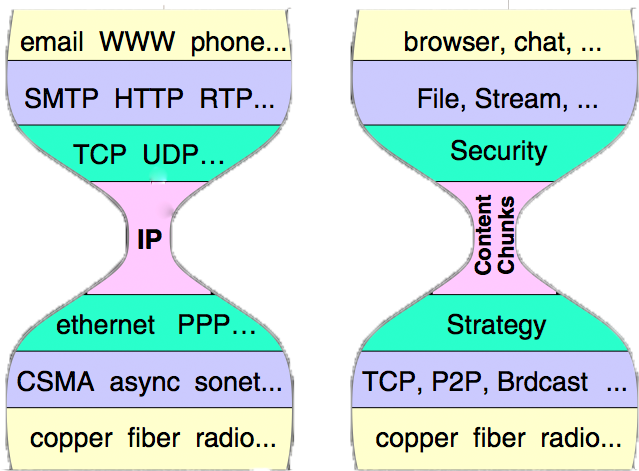
\includegraphics[width=0.5\textwidth]{NDNhourglass.png}
	\caption{TCP/IP协议栈和CCN协议栈的对比}
	\label{fig:ProtocolStacks}
\end{figure}
\par
协议栈中数层体现了两者之间的相似性,比如第二层的成帧协议体现了物理链路中发送方、接收方之间的协商;第四层传输层协议体现了数据或服务的请求者、提供者之间的协商。承上启下,为双方提供统一接口的第3层,即网络层,体现了IP协议成功的许多因素。首先,网络层对链路层提供的服务的需求很低,是无状态、不可靠、不保序、尽力而为的。CCN的网络层(即第三层),在这一点上和IP是吻合的,即不对链路层提供的服务提出过高要求。这一点为其保留了IP较多优点。同时值得一提的是,CCN也可以作为其它协议或架构的负载,包括作为IP的负载。
\par
CCN在许多关键点上不同于IP。其中两者是策略和安全。两者均为NDN协议栈中新出现的层。CCN可以最大化利用同时存在的多个连接,比如以太网、3G、蓝牙和802.11,因为CCN和第二层的关系更加简单。策略层在变化的外界条件下,根据多个同时存在的连接,做出详细的、动态的优化,从而最大化的利用多个连接。安全层保障数据本身是受信任的,而不是数据所经过的通路是受信任的,由此避免了安全策略上IP网络的许多问题。

\subsection{设计理念}
\par
CCN网络通信是由数据请求方驱使的。网络中有两种包,数据请求(Interest)和数据应答(Data)。数据请求方向本地的所有连接广播数据请求,任何收到数据请求,并且有名称满足要求的数据的节点可以应答。数据应答包的发出都是由收到特定的请求所触发,换言之,数据应答包都是为了满足特定的请求。
\par
当且仅当数据请求包的名称是数据应答包的名称的前缀子串(Name prefix)时,数据应答可以满足数据请求。CCN名称是层次结构的,所以前缀的吻合可以描述为数据应答包的名称是数据请求包的名称的子树。IP用同样的方式来解析树状的IP地址,即<网络地址,子网地址,主机地址>。IP的经验表明,这样的方式可以实现路由表树型的高效压缩和快速查找。名称前缀也是当前环境相关的。
\par
CCN节点的工作方式和IP节点是类似的:节点收到数据包,进行最长前缀匹配,并由匹配结果决定下一步行动。图\ref{fig:NodeLogic}是CCN节点模型的结构图,该图体现了一个CCN节点包含的数据结构,和在收到一个特定数据请求时进行的动作。其中主要有三个数据结构:前递表(Forwarding Information Base, FIB),数据缓存(Content Store, CS)和待应答表(Pending Interest Table, PIT),会在下文作出介绍。\cite{NDNDSRef}
\begin{figure}[h!]
	\centering
	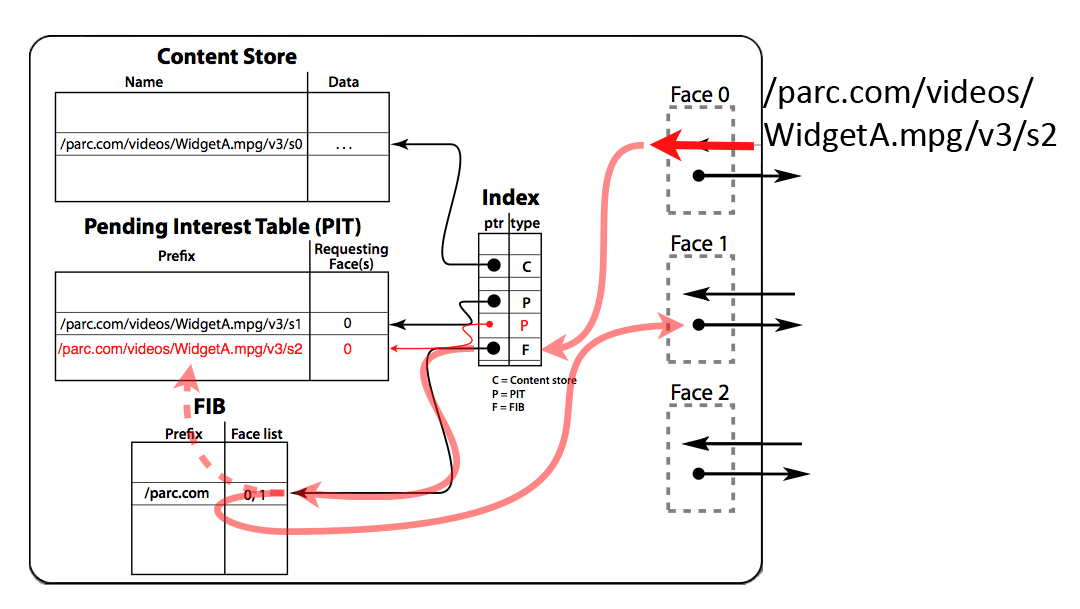
\includegraphics[width=0.9\textwidth]{CCNnodemodel.png}
	\caption{CCN节点模型}
	\label{fig:NodeLogic}
\end{figure}
\par
前递表的作用是将数据请求传递向可能有对应的数据应答的节点。其与IP的路由表相近,但是允许一个表项和多个接口进行匹配,而不是对于每一个接口,存在一张路由表。这一点体现了CCN不局限于基于一颗生成树的前递,其允许一个节点同时对多个连接的数据源进行请求,多个数据源也可以同时处理收到的请求。
\par
数据缓存和IP路由的缓存作用近似,但是替换策略不同。由于每个IP包包含了源和目的地址,其对于别的点之间的交互是不起到作用的。因此,IP路由器在将收到的包写入缓存,然后转发出去之后,就可以将该包擦除(利用最近使用(MRU)替换)。CCN包是与请求端点无关,因而每一个包有可能可以满足多个用户的数据请求,只要数据请求的名称匹配。
\par
待应答表保存了向数据提供方前递的数据请求(上行请求),因此当收到数据提供方的应答时,可以根据待应答表中的记录将数据应答传送给数据请求方。因此,在CCN中,只有数据请求包在上行时经过路由,并在经过路由节点的同时留下一系列的记录,下行的数据应答包可以根据路由节点的记录找到数据的请求者。在路由节点收到下行数据应答后,其将所收数据应答对待应答表中的对应表项中的所有节点进行多播,并且擦除该表项。长时间没有收到数据应答的数据请求会超时,而如果数据请求方仍然希望请求该数据,请求方应当负责重新发送数据请求。
\par
当数据请求包到达某节点的某接口后,节点首先进行名称的最长前缀匹配。上述数据结构的查找是有序的,数据缓存的匹配优先级高于待应答表,高于前递表。数据请求的处理逻辑如图\ref{fig:InterestLogic}所示。
\begin{figure}[h!]
	\centering
	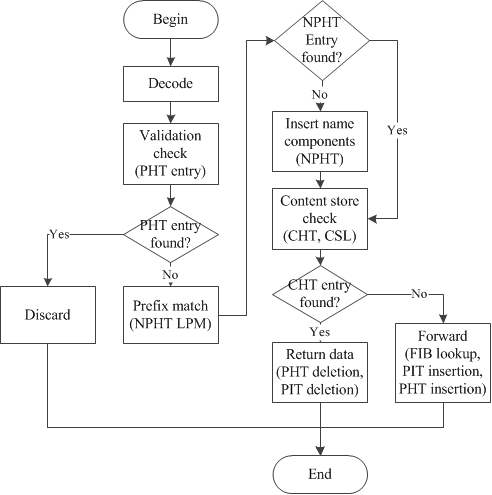
\includegraphics[width=0.75\textwidth]{InterestLogic.png}
	\caption{收到数据请求的处理逻辑}
	\label{fig:InterestLogic}
\end{figure}
\par
因此,在一个节点收到请求后,如果数据缓存找到了满足请求的数据,会直接返回该数据,同时收到的请求由于已经被满足而会被丢弃。
\par
如果数据缓存没有前缀匹配项,而待应答表中有名称完全匹配项,收到请求的接口会被加入到路由节点待应答表中该名称的下行接口表上,同时收到的请求会由于别人已经在请求同名数据,且别人的请求已经向数据源上行而被丢弃。这时路由节点所要做的只是当数据应答到来时,将数据应答也向这个数据请求的接口发送一份。
如果二者都没有匹配项,而前递表有匹配项,则数据请求根据前递表的匹配项上行。收到请求的接口将会被从前递表匹配项上移除,如果前递表匹配项此时仍不为空,则对于其所记录的每一个接口发送该数据请求。并以收到请求的接口,创建一个新的待应答表项。
\par
如果三者都没有匹配的表项,则丢弃该数据请求,因为收到请求的路由节点既没有满足要求的数据,也不知道该向哪里前递已获取满足要求的数据。
\par
数据应答包的处理要相对简单。由于数据应答包不经过路由,而是直接根据待应答表进行下行,在收到数据应答时,首先进行名称的最长前缀匹配。如果数据缓存有匹配项,则收到了重复的数据,予以丢弃。如果前递表发现了满足项,则说明待应答表中没有满足项,说明数据没有请求者,是不需要的,予以丢弃。如果带应答表中发现满足项,则(可选的)进行数据核实和写入数据缓存,之后根据待应答表的满足项移除收到数据应答的接口后,对满足项中的其它接口进行下行。
图\ref{fig:DataLogic}反映了数据应答的处理流程。不同于IP先入先出的缓存模型,CCN缓存模型允许整个网络的节点缓存实现透明缓存。所有节点可以根据自己的能力和策略进行缓存。
\begin{figure}[h!]
	\centering
	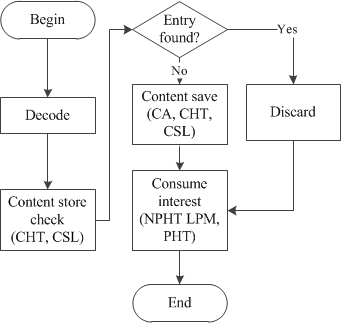
\includegraphics[width=0.50\textwidth]{DataLogic.png}
	\caption{收到数据应答的处理逻辑}
	\label{fig:DataLogic}
\end{figure}
\par
通过数据请求指定的多点数据回取的特点使得CCN在变化快速的环境下依然可以灵活应用。任何处在多个网络中的节点可以作为其所处的多个网络之间的缓存和路由。利用其缓存,一个移动的节点可以作为多个彼此不相连区域进行连接的媒介,或者为不连贯的链路提供延迟的连接。

\section{命名数据网同步模型}
\par
同步问题(Synchronization)在文件共享服务,实时聊天应用等等多个用例中有实际应用。多人联机游戏也是用例之一。自组织的多人联机游戏的每一个节点都在运行一个对等的独立实体,每一个节点都对自己的实体负责的游戏对象有决定权,并能发布关于它们的数据更新。对于自己没有决定权的对象,游戏实体应该通过网络接收数据更新,从而保持各个游戏实体间信息的一致性,即同步。
\par
同步问题同是也是NDN网络研究的重要问题。虽然为了提供更广的支持,NDN仍然拥有“只从数据发布源获取数据”的功能,但是由于弱化了数据存储位置的概念,能体现NDN思想的设计思路并不利用该功能。由此带来的问题是,多个节点的数据希望保持一致时,一般不存在某一特定中心节点,或是数据的最初提供者,可以为别的节点的数据负责;换言之,不存在服务器可以为多个客户端提供一致的数据。因此,发布数据的端点如果希望别的端点可以获得更新的数据,应该通过命名空间的设计,无二意的对其发布的数据进行命名 。
\par
CCN在提出时包含了最基础的同步设计方案,本文将在下面进行概述。然而该基础思路存在许多问题,为了更高效的实现同步,NDN小组提出了ChronoSync\cite{ChronosRef},其特点也会在下面进行概述。
\subsection{CCNx的同步协议}
\par
CCNx的同步协议\footnote{在线文档,http://www.ccnx.org/releases/latest/doc/technical/SynchronizationProtocol.html}
是针对知识库的片(Repository slice)的。知识库片的组织是根据名称的层次结构形成的一颗树。对于需要同步的每一片,一个同步实体一直保持运行。对于树中的每一个节点,同步实体记录其名称和内容的哈希值。对于叶子节点,其哈希值是对应的数据内容根据选定的哈希算法,例如SHA256,得到的消息摘要(Message Digest)。中间节点和根节点的哈希值是所有子的哈希值的加和。
\par
由此,每当同步实例收到别的节点发出的有关根节点的哈希值的数据请求(root advise interest)时,同步实例可以和本地的根节点哈希值进行比较。如果值不同,则同步实例可以按照树形结构向下寻找到出现不同值的底层节点,然后对该节点发出节点数据请求(node fetch interest),或是直接对根节点发出节点数据请求,从而获得对方不同的数据内容。
\par
此方案是进行树形数据结构同步的最直接方法。其实现起来较为简单,但是具有几个突出的问题。首先,树的内容只可以增,不可以减。仅此一点就使得其直接应用在我们的用例中变得不现实。其次,同步的开销比较大。每一次出现根节点状态的不同,就需要重新传输、构建整棵树,或是用多个往返时间找到不同出现的位置。
\par
CCNx  Sync只是NDN同步问题解决方案的雏形,近两年实现的ChronoSync是该方案的改进。
\subsection{ChronoSync}
\par
ChronoSync是CCNx Sync方案的改进。同步的对象不再是知识库片中的整个名称树,而是应用决定的特定数据集(Dataset)。
\par
ChronoSync利用预定的哈希算法,例如SHA256,计算数据集内容的哈希值作为数据集的状态,并将状态的同步和数据集内容的同步区分开来。\cite{ChronosRef2}
\par
几个需要对分布式存储的数据集进行同步的节点定期发出名称中包含自己的数据集状态的数据请求,接收到数据请求的节点比较收到的状态和本地的状态是否相同,如果不同,则可以返回本地的数据集内容作为数据应答,数据请求的发出者可以根据预定的规则和当前的情况决定是否接受数据应答中包含的数据作为当前时刻正确的数据。
\par
为了帮助多个节点做出决定,同时减少数据应答中应该包含的内容,每个节点维持一个状态历史,记录本地经历过的每一个状态和对应的数据内容的变化。如果收到的数据请求中包含的状态在自己的状态历史(digest history)中,则该节点只需要回复该状态点之后的数据内容变化。另外,如果自己发布了别的节点应该接受的新内容,如果发布的内容变化不大,则可以将其直接夹带(piggyback)在数据请求中,同时告知数据请求的接受方直接应用该该变化。如果历史和夹带都没有帮助节点直接获得或决定是否应用变化,则更新的过程退化为普通的NDN数据请求、数据应答交互,不再属于同步模块的考虑范畴。
\par
除此之外,为了应对新加入者的情况和网络可能出现的分块等的异常,ChronoSync加入了恢复(recovery)机制,在收到恢复数据请求后,数据应答将包括用整个数据集,以帮助请求者快速重建状态历史。
一个简单的用例是多人聊天程序ChronoChat\footnote{项目源码,https://github.com/named-data/ChronoChat}。
\par
在此用例中数据集是所有人在所有时刻发出的聊天信息。

\section{命名数据网开发者函数库}
\label{CCLSection}
\par
NDN项目为应用开发者提供一套高级语言的开发接口,即开发者或客户端函数库(Common Client Library)。函数库接口在在线文档\footnote{在线文档地址,http://named-data.net/doc/ndn-ccl-api/}可以找到。
\par
虽然NDN对于底层(例如链路层)协议的实现已经有了规划,但是为了和当前的硬件环境保持兼容,NDN通信的实现仍然是作为传输层协议的负载的。因此,客户端函数库由Java、Python、C++等高级语言实现。就传输方式而言,NDN客户端函数库直接利用这些高层语言所包含的传输层接口的实现,NDN流量将以NDN协议的格式进行解析,但以TCP或UDP协议为负载进行通信。
\par
由于本文开发的应用使用的引擎,Unity3D\footnote{参考,http://unity3d.com/},是基于DotNet平台的。而当前的NDN开发者函数库并没有针对DotNet的实现,因此本文作者的工作也包含了与ndnd-tlv兼容的NDN开发者函数库的开发。在此简单介绍从NDN应用开发角度上会接触到的几个类。
\par
接口(Face)类:接口类封装了一个存在的网络接口。注册兴趣和发出兴趣的针对的对象为接口。即RegisterPrefix和ExpressInterest都是Face类的方法。
\par
节点(Node)类:节点类记录了所有的接口。在接口RegisterPrefix或是ExpressInterest时,实际上是通过Node的同名方法调用操作系统收发函数实际进行收发的。
\par
数据请求处理类(OnInterest,OnRegisterFailed):应用开发者通过继承数据请求处理类,为其中的虚方法提供重载,对收到的数据请求或是节点发出的注册失败通知进行处理。
\par
数据应答处理类(OnData,OnTimeout):应用开发者通过继承数据应答处理类,为其中的虚方法提供重载,对收到的数据应答或是节点发出的请求超时通知进行处理。
\section{游戏联机技术}
\par
多人游戏联机主要采用两种模型。早期的互联网游戏的联机是点对点的,每个节点所运行的是一个独立的游戏实体,通过同步使得多个独立游戏实体在每一个时间点保持相同。这样的游戏有帝国时代1、2以及星际争霸1,而这些游戏也成为早期研究的对象\cite{IPMOGInfo}。早期点对点技术带来了许多问题,例如实际传输流量更大,联机速度由连接速度最差的端点决定。
\par
游戏Quake引入了客户端/服务器的联机架构。每个节点所运行的应用只起到用户接口的作用,即通知服务器用户的输入,并对服务器返回的数据进行渲染。所有的决定权在服务器端, 信息的处理也在服务器端完成。如此架构遇到的主要问题是延迟。用户在赋予自己的角色前进指令后,需要等到一个往返时间之后服务器的确认才可以在本地体现角色的前进。为了解决该问题,Quake 2游戏的引入了本地渲染器的预测技术。对于上述的用例,本地会预测服务器端的确认,并作出渲染。该技术同时引入了对错误预测的处理\footnote{在线文档提供了更详细的描述,http://gafferongames.com/networking-for-game-programmers/what-every-programmer-needs-to-know-about-game-networking/}。
\par
近10年来游戏联机的C/S模型逐步成熟,并应用在主流商业化的大型MMORPG游戏中。然而其服务器端的流量汇聚,和服务器单点出现问题会导致服务不可用的问题依然没有得到解决。因而近年来仍有许多研究机构提出了基于DHT等技术的IP网络下点对点自组织的游戏实现\cite{IPP2PMMORPG,IPP2PMMORPG2,IPP2PMMORPG1}。

\section{k最近邻居相关的数据结构}
\label{kNNIntroSection}
\par
kNN问题是游戏同步问题中虚拟环境局部性要求的抽象化描述。
\par
由于整个游戏的虚拟空间可能过大,其中包含的节点过多,希望每一个节点获取整个虚拟空间的全部状态信息是不现实的。同时由于游戏本身的要求,每个节点只需要获取在它的感知范围内的其它对象,即为游戏虚拟环境的局部性要求。该要求可以理解为,每个节点在任一时刻只希望了解自己的k-近似最近邻居。此要求在系统需求分析中也有详细的叙述 (ref)。
\par
本文还将kNN问题所使用的数据结构分为静态和动态,二者分别应对物理节点不动和移动的情况。

\subsection{树形结构}
\par
以树形结构为例。经典的可以用于kNN查找的静态树结构有kd树,R树 。然而对于节点会移动的情况,如果仍然采用经典的静态树结构例如kd树或R树,为了保证树形结构的效率,树需要动态的进行平衡(balance)。为了简化或是避免平衡的过程,基于这些基础的静态树结构,研究者提出了TPR树等动态树。虽然介绍kd树的kNN查找过程会有助于方案和优化的理解,但是出于篇幅的限制,本文并不概述kd树或是R树等基础数据结构。
\par
除此之外,树形结构的节点和几何区域的表示问题中所使用的树传统意义上有两种。一种的节点为区块,称之为区块树(Trie-Based Tree);另一种的节点为物理节点,或是多个物理节点的一定意义下的结合(该特定意义也可以是包含这些节点的区块,在此意义下两者的不同体现在叶子节点的含义以及平衡的过程),称之为节点树(Point-Based Tree)。本文后来所使用的八叉树是区块树中的一种。

\subsection{位置敏感哈希}
\par
位置敏感哈希是高维数据降低维度的方案之一。位置敏感的哈希函数的定义如下\cite{LSHRef}。
\begin{definition}
位置敏感哈希:\rm 一簇$H = { h : S \to U }$的哈希函数被称为是距离定义$D$上$(r_1, r_2, p_1, p_2)$位置敏感的,当且仅当$ \forall v,q \in S $且$ p_1 > p_2 $,$ r_1 < r_2 $,
\begin{itemize}
\item如果$ v \in B(q, r_1), $则$ Pr_H[ h(q) = h(v) ] \geq p_1$;
\item如果$ v \notin B(q, r_2), $则$ Pr_H[ h(q) = h(v) ] \leq p_2$。
\end{itemize}
\end{definition}
\par
对于本文采用的欧几里得距离定义的p稳定的位置敏感哈希而言,一种常见的思路是用如下两个步骤进行维度缩减。
\par
假设输入的维度为$n$的向量$(x_1, x_2, \dots x_n)$。从一簇位置敏感哈希函数中随机选取$L$个,对于每一个$ j = 1 \dots L $,
\begin{equation}
h_j = ( \sum_{i=1}^{n} a_{ij} \cdot x_i ) \bmod Size
\end{equation}
\par
其中$a_{ij}$是满足2维稳定分布的一个随机矩阵;$Size$是第一步哈希桶的个数。在得到了一组$h_j$后,
\begin{equation}
H(x_1, x_2, \dots x_n) = ( \sum_{i=1}^{L} b_i \cdot h_i ) \bmod P
\end{equation}
其中$b_i$是满足2维稳定分布的一个随机向量;$P$是第二部哈系桶的个数;$H(x_1, x_2, \dots x_n)$为最终得到的哈希结果。
\par
本文在提出对比方案时,首先是按照上述公式进行操作的,然而之后的测试发现效果并不良好,原因和分析在\ref{ComparisonSection}有所说明。
\section{名称集表示相关的数据结构}
\par
为了更高效的实现同步,在不需要数据更新时不进行更新,在本文的设计方案中每一个数据请求包含了本地实体的消息摘要,或状态。状态有多种方式体现。以下是两种实际方案,其优劣在理论分析部分(ref)也有所记述。
\subsection{加密式哈希}
\par
本文中哈希的作用是用较短的定长的二进制数据表示很长的变长二进制数据的方法,又称为消息摘要(Message Digest)。本文涉及到的哈希函数是加密式的(Cryptographic Hash),哈希前后的数据没有任何直接联系。
\par
如果哈希后的数据长度有所保证,例如采用SHA256作为哈希函数时,基本可以认为不同的数据得到相同的哈希值的可能性极小。综上, 除了用于比较两个较长的变长二进制数据是否相等外,该哈希没有其它明显意义。
\par
常见的摘要函数有MD5,SHA1,SHA256,SHA512等。另外值得一提的是,为了保证哈希前后的数据没有联系,上述哈希算法的计算过程较为复杂。本文的用例是将一组字符串哈希到一个16位或32位整型,本用例中可以采用更简单的哈希函数,例如FNV哈希或是Murmur哈希。
\subsection{可逆转的Bloom Filter}
\label{IBFIntroSection}
\par
可逆转的Bloom Filter(Invertible Bloom Filter)\cite{IBFRef}是普通Bloom Filter的改进版,除了拥有普通Bloom Filter有假阳性(False positive)概率的体现集合是否在元素中的功能外,IBF有较高的概率将两个集合中不同的以名称表征的元素恢复出来。其基本工作过程和原理如图\ref{fig:IBF}所示。图中集合A、B分别拥有名称集\{a, b\}和\{a, c\},假设经过特定的3个哈希,它们分别落在如图中的几个桶内;通过将二者的IBF做差,可以恢复出二者集合的不同元素,即b和c。
\begin{figure}[h!]
	\centering
	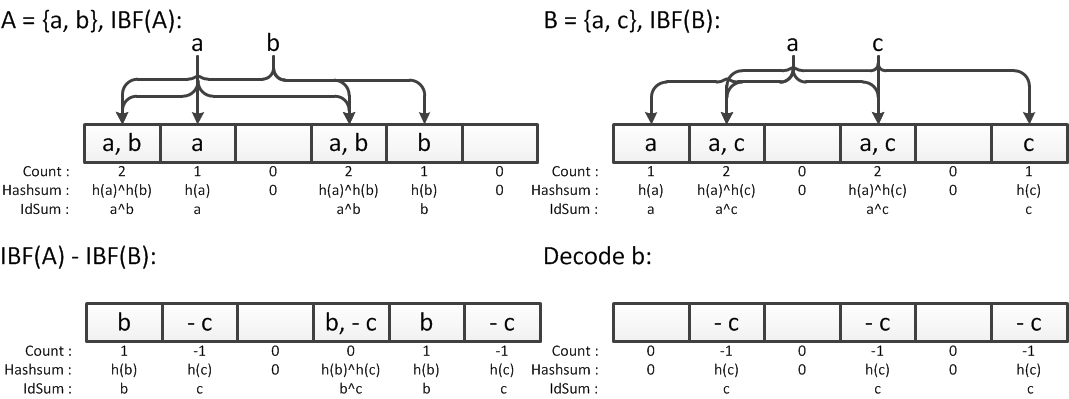
\includegraphics[width=0.9\textwidth]{InvertibleBloomFilterDemo.png}
	\caption{IBF的工作过程}
	\label{fig:IBF}
\end{figure}
\par
IBF在Bloom Filter\footnote{介绍,http://en.wikipedia.org/wiki/Bloom\_filter}的基础上为每个桶添加了和字段以及和哈希字段,并为和哈希字段提供了利用异或求和的方法,从而使得通过将两个IBF做差(同样是异或),将有较高的概率恢复出得到IBF的两个集合之间的不同。这里受到篇幅限制,无法详细描述IBF的工作流程以及大小随恢复差集的概率的关系。
\par
IBF作为对比方案,其应用体现在文中的理论分析\ref{IBFComparisonSection}部分。
\section{开发引擎Unity3D}
\par
本文开发的游戏应用采用的时Unity3D引擎。该引擎为了兼顾不同的平台,采用了DotNet架构的开源实现Mono Framework。目前该引擎仍然基于Mono 2.6\footnote{官方站点,http://www.mono-project.com/Main\_Page}版本,因此并未提供对DotNet 4.0的特性的支持。该引擎提供了从C\#,语法上类似Javascript的UnityScript,以及自定义语言Boo到IL的编译工具。本应用和为应用提供支持的开发者函数库采用的是C\#编程语言,编译链接的DotNet版本为2.0。
\par
在该游戏引擎中,游戏的对象存储在按照名称索引和组织的一棵树中。
\section{本章小结}
\par
本章描述了论文中所使用的主要技术,和其与论文设计方案、优化方案、对比方案的联系。命名数据网是设计方案基于的网络架构;已知的同步模型是本文方案的参照和对比;开发者函数库是本文工作的另一个需求和开发的基础;游戏联机技术是本文研究的对象,其IP下的实现是本文的对比;kNN问题和Digest的表示与本文的设计决定和对比方案或是优化有关系。为了帮助充分理解文章在设计方案中做出的选择和考虑,本章对CCN架构和同步模型的描述较为详细。
% multiple1902 <multiple1902@gmail.com>
% intro.tex
% Copyright 2011~2012, multiple1902 (Weisi Dai)
% https://code.google.com/p/xjtuthesis/
% 
% It is strongly recommended that you read documentations located at
%   http://code.google.com/p/xjtuthesis/wiki/Landing?tm=6
% in advance of your compilation if you have not read them before.
%
% This work may be distributed and/or modified under the
% conditions of the LaTeX Project Public License, either version 1.3
% of this license or (at your option) any later version.
% The latest version of this license is in
%   http://www.latex-project.org/lppl.txt
% and version 1.3 or later is part of all distributions of LaTeX
% version 2005/12/01 or later.
%
% This work has the LPPL maintenance status `maintained'.
% 
% The Current Maintainer of this work is Weisi Dai.
%

\chapter{系统需求分析}
\echapter{Analysis}
\label{AnalysisChapter}
\section{系统需求}
\begin{itemize}
\item
局部性(Locality)
\par
根据游戏设计,每个节点应当具有一个球形的感知范围(Area of interest)。节点应当只收到落在自己的感知范围内的对象的位置和行动的更新。不仅如此,如前\ref{kNNIntroSection}部分所述,由于整个游戏的虚拟空间过大,其中包含的节点过多,希望每一个节点获取整个虚拟空间的全部状态信息是不现实的。此要求即为游戏虚拟环境的局部性要求。该要求可以理解为, 网络中每个节点请求、收到的内容应当尽可能的对自己有用,且尽可能的少。局部性是避免广播的内容过多,网络流量过大,从而减少延迟的重要要求。
\par
局部性的要求在物理环境和虚拟环境的反映可以用图\ref{fig:Locality}描述。
\begin{figure}[h!]
	\centering
	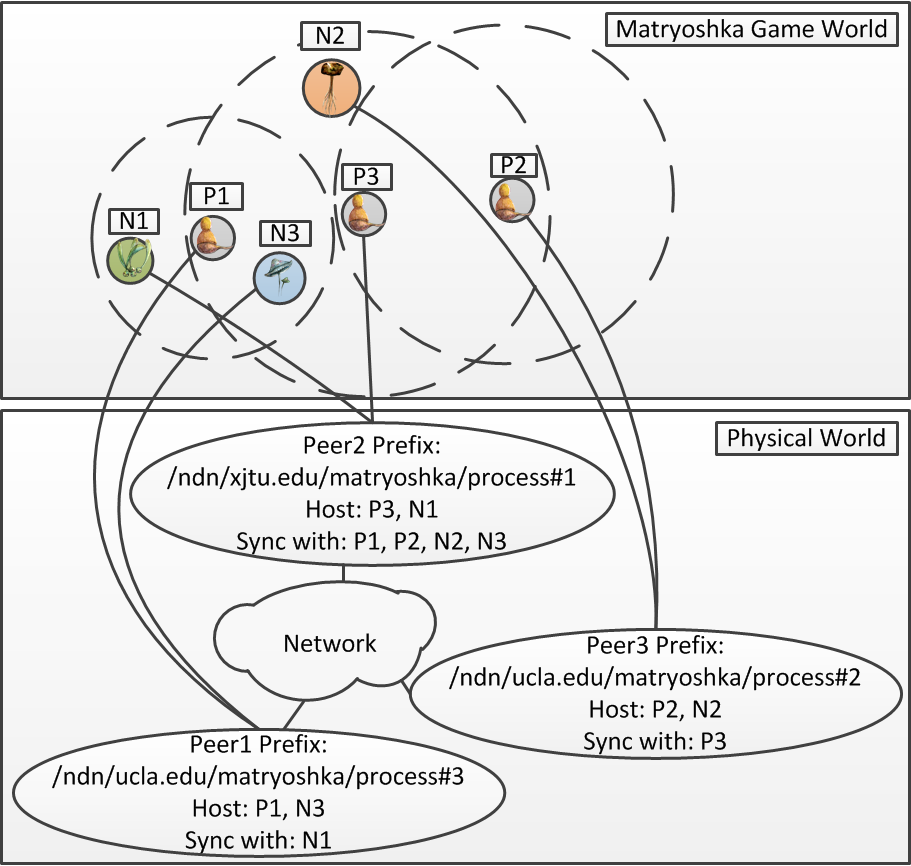
\includegraphics[width=0.75\textwidth]{ProblemDemo.png}
	\caption{游戏应用的局部性要求}
	\label{fig:Locality}
\end{figure}
\par
图\ref{fig:Locality}体现了分布式虚拟环境。P3应该发现P1、P2和N2、N3。P1、P2分别由Peer1和Peer3主持。对于这样的情况,Peer2如何通过向网络进行询问,了解到上述四个点的信息或名称,而不包括N1的信息,即为局部性要求的体现。
\item
实时性(Realtime-ness)
\par
当对象移动或是做出动作时, 每个对其感兴趣的节点,即包含该对象在自己的感知范围内的节点,应当尽快的获得关于移动或是动作的更新。特别是当一个对象从一个节点的感知范围外移动到感知范围内,或是从感知范围内移动到感知范围外,即加入和离开事件发生时,节点应该尽可能早的获悉事件的发生。
\item
大规模可拓展性(Scalability)
\par
由于本项目旨在解决大规模网络游戏的联机问题,只要不是用户主观需求,所有节点应当尽可能的处于同一个虚拟世界中,因此大规模可拓展性是设计方案中需要考虑的。这一点体现在NDN网络中即为尽可能多的利用节点的数据缓存中的信息,通过全局共享的命名空间,实现在满足实时性的同时存在最大规模的数据共享。
\item
健壮性(Robustness)
\par
在实际网络环境中,分块、丢包、乱序、掉线等异常时有发生。由于当前的客户端函数库是基于TCP协议的,协议本身对传输质量有保证,这些情况的发生并不应该起到很大影响。但是,考虑到TCP协议的头部较大,影响传输效率,实际实现会采用UDP协议。同时,理论NDN架构并不基于TCP,理论NDN网络层也是无状态的,不提供针对丢包、乱序的处理。综上,更高层的协议,即游戏应用通讯的应用层协议,应当为这些异常情况负责。游戏应用应当在出现丢包、乱序时尽可能的自行做出处理,并在侦测到对象掉线后予以删除。
\end{itemize}
\section{系统框架}
\par
需求分析中根据系统的逻辑功能,将系统划分为如下几个模块。
\begin{figure}[h!]
	\centering
	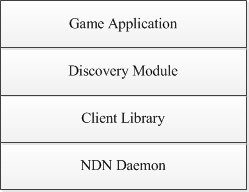
\includegraphics[width=0.40\textwidth]{ApplicationStructure.png}
	\caption{系统框架层次图}
	\label{fig:AbstractStructure}
\end{figure}
\par
\begin{itemize}
\item
NDND(NDN Daemon)
\par
运行在各个节点负责NDN路由等节点逻辑的NDN进程。当前最新的NDND是NFD\footnote{NFD的介绍和源码,https://github.com/named-data/NFD},本应用支持的时ndnd-tlv\footnote{ndnd-tlv的介绍和源码,https://github.com/named-data/ndnd-tlv},本应用早期的版本基于的是ccnd\footnote{ccnd的介绍和源码,https://github.com/ProjectCCNx/ccnx}。
\item
开发者函数库
\par
如前面所介绍,开发者函数库为NDN应用封装了NDN提供的功能。
\item
同步模块
\par
同步模块是在开发者函数库之上,独立于游戏应用之外的函数库。同步模块实现分布式虚拟环境的发现、更新的功能。将同步模块分离的意义的在于别的类似功能的应用可以直接使用该模块,而不必担心和游戏应用的耦合。
\item
游戏应用
\par
游戏应用负责渲染、插值、预估等功能。其调用同步模块提供的功能,决定渲染哪些对象。
\end{itemize}
\section{本章小结}
本章描述了系统的四大需求,局部性、实时性、可拓展性和健壮性。在此之后,本章给出了系统的大致框架,本文需要实现的主要部分在于框架的上三层,需要设计的部分在于框架的上两层。下面的本文的重点将在同步模块的设计、评估和改良上。


% multiple1902 <multiple1902@gmail.com>
% design.tex
% Copyright 2011~2012, multiple1902 (Weisi Dai)
% https://code.google.com/p/xjtuthesis/
% 
% It is strongly recommended that you read documentations located at
%   http://code.google.com/p/xjtuthesis/wiki/Landing?tm=6
% in advance of your compilation if you have not read them before.
%
% This work may be distributed and/or modified under the
% conditions of the LaTeX Project Public License, either version 1.3
% of this license or (at your option) any later version.
% The latest version of this license is in
%   http://www.latex-project.org/lppl.txt
% and version 1.3 or later is part of all distributions of LaTeX
% version 2005/12/01 or later.
%
% This work has the LPPL maintenance status `maintained'.
% 
% The Current Maintainer of this work is Weisi Dai.
%

\chapter{系统设计}
\echapter{Design}
\label{DesignChapter}
本系统的设计包含两个主要部分。客户端函数库的设计和应用层同步、发现、更新模块的设计。由于同步模块的功能是获取对象的名称,本文中有时也将其称为发现模块。由图\ref{fig:AbstractStructure}所示,客户端函数库为发现模块提供和操作系统、以及NDN底层组件交互的接口;而发现模块为游戏提供发现节点,更新位置的功能。

\section{客户端函数库}
\par
NDN客户端是NDN项目的重要组成部分。其为开发者提供一套和NDN的底层组件交互的接口。例如,客户端函数库对上层应用开发者应当提供“注册数据请求名称前缀(Register Prefix)”函数。函数的具体实现,如何调用语言和操作系统提供的传输层网络接口,以及和NFD的交互过程应当在客户端函数库中实现。
\par
目前的NDN客户端函数库的实现有Java,Python和C++三种语言。由于Unity3D引擎的语言选择是基于Mono Framework的,作者的工作还包括客户端函数库的C\#语言实现。
\par
设计上所有NDN客户端函数库应当提供统一的接口,遵循统一的规定。具体规范在项目的在线文档有所描述(ref)。目前的Java语言NDN客户端函数库的类图结构如图\ref{fig:CCLClassDiagram}。作者开发的C\#客户端函数库遵循同样的类图结构。
\begin{figure}[h!]
	\centering
	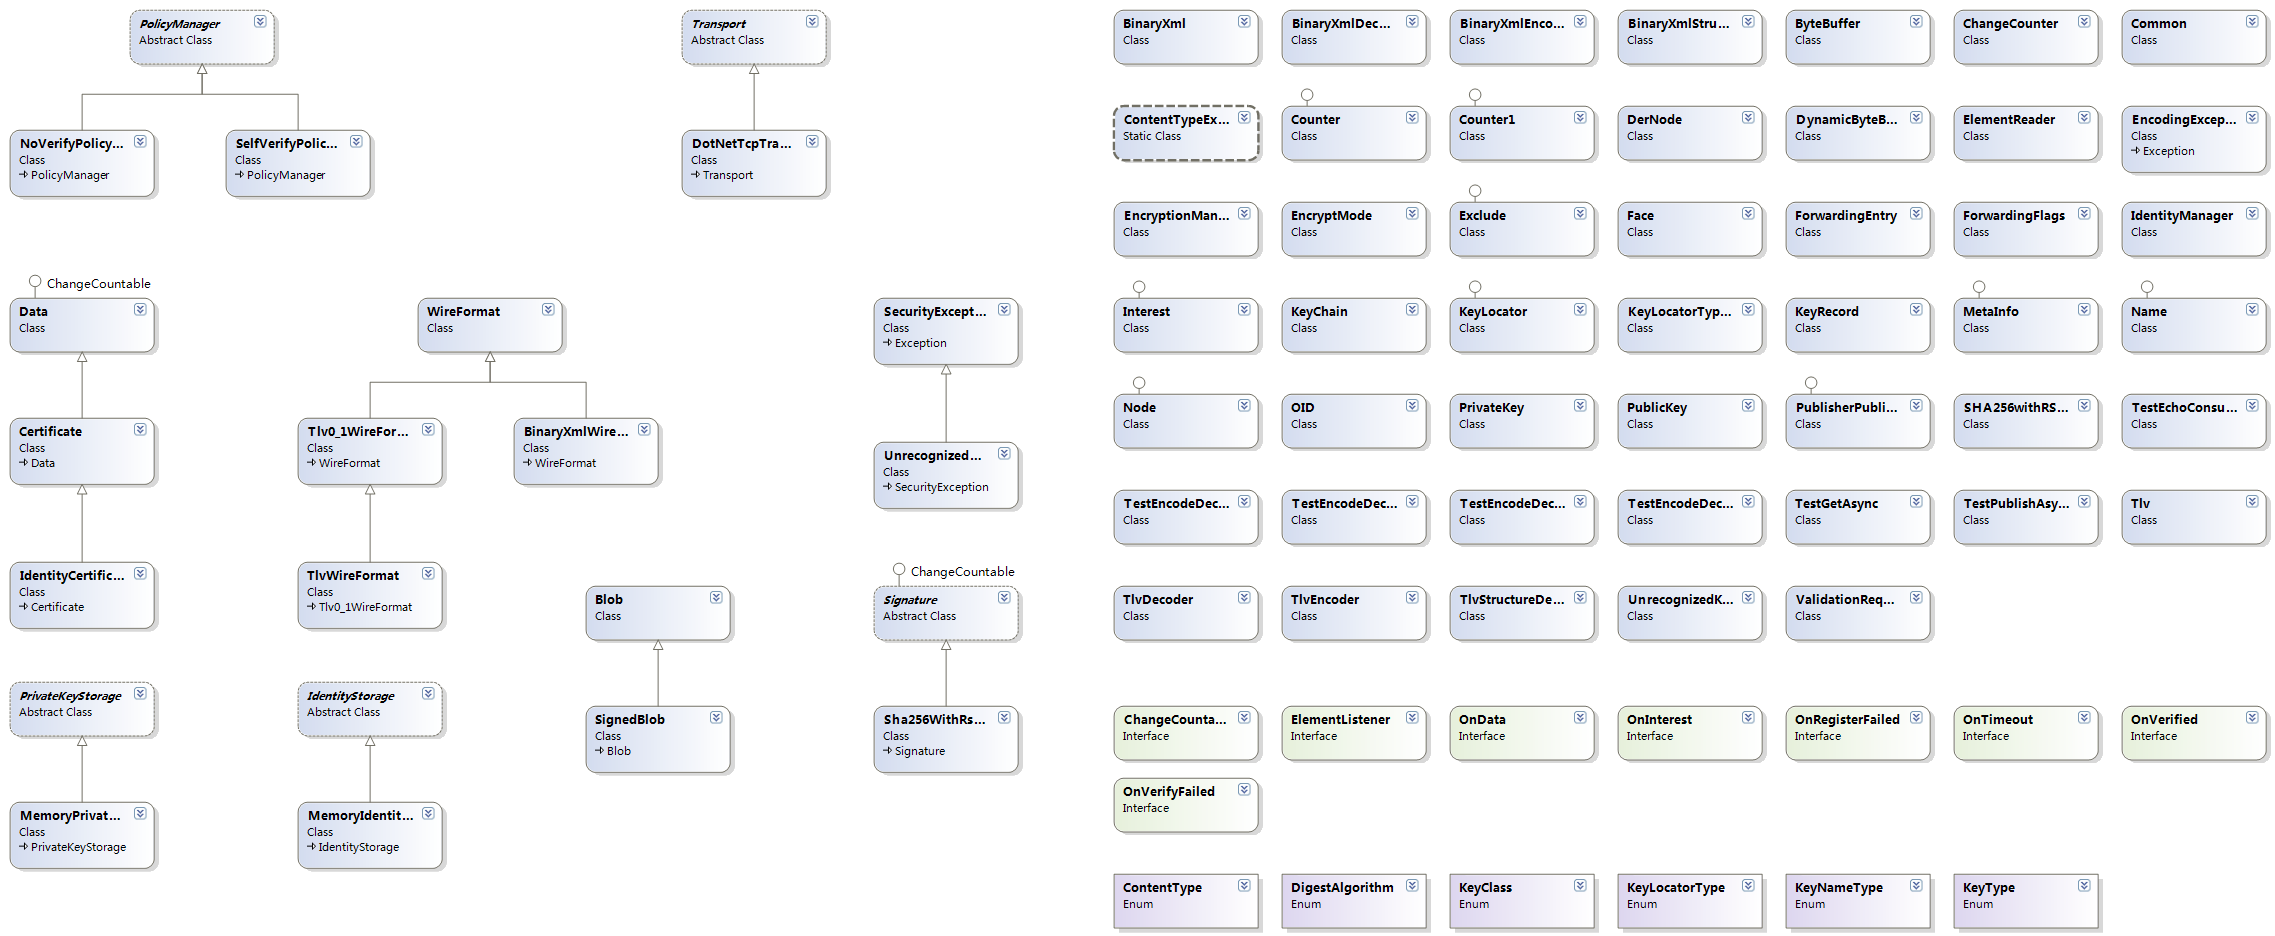
\includegraphics[width=0.95\textwidth]{TranslatedJndn.png}
	\caption{开发者函数库的类图描述}
	\label{fig:CCLClassDiagram}
\end{figure}
\par
由于篇幅限制,各个类的成员、方法和功能在此无法一一展开或描述,而简单应用开发中使用的重要的类在\ref{CCLSection}中已经有所介绍,在此不再赘述。

\section{设计详述}
\par
本部分详细叙述应用设计和工作流程。
\par
NDN应用设计的重要环节是命名空间(Namespace)的设计,为了达到局部性和可拓展性的目标,提供全局共享的命名空间是必要的。同时,由于NDN交互是通过数据请求和数据问答实现的,应用设计中应当考虑的问题是节点应该问网络怎样的问题,从而既在表达上没有二义性,又能尽量多的提供路由可用的信息,减少广播,提高效率。
\par
在游戏应用的同步用例中,对于每个节点,两个自然的问题是谁在我的附近,和它在哪里,在做什么。两个问题的结构对应着两个步骤,其优势在于, 问题一为问题二提供有助于路由的节点名称,从而经过网络节点模型的优化后,问题二的实际传输类似于单播。对于问题一,为了发现哪个对象在给定节点的附近,定期的广播数据请求是必要的。为了使命名空间可以共享,本文采取了对整个虚拟空间的静态八叉树划分。对于问题二,本文利用传统的NDN请求、应答交互实现位置、行动的更新。
\subsection{八叉树划分}
\par
虚拟环境的八叉树(Octree)\cite{OctreeRef}划分将整个三维虚拟环境划分为八个均等的立方体,对于每个立方体将其均等的划分为八个更小的立方体,以此类推,直到达到提前预设的层数。图\ref{fig:Octree}展示此划分。
\begin{figure}[h!]
	\centering
	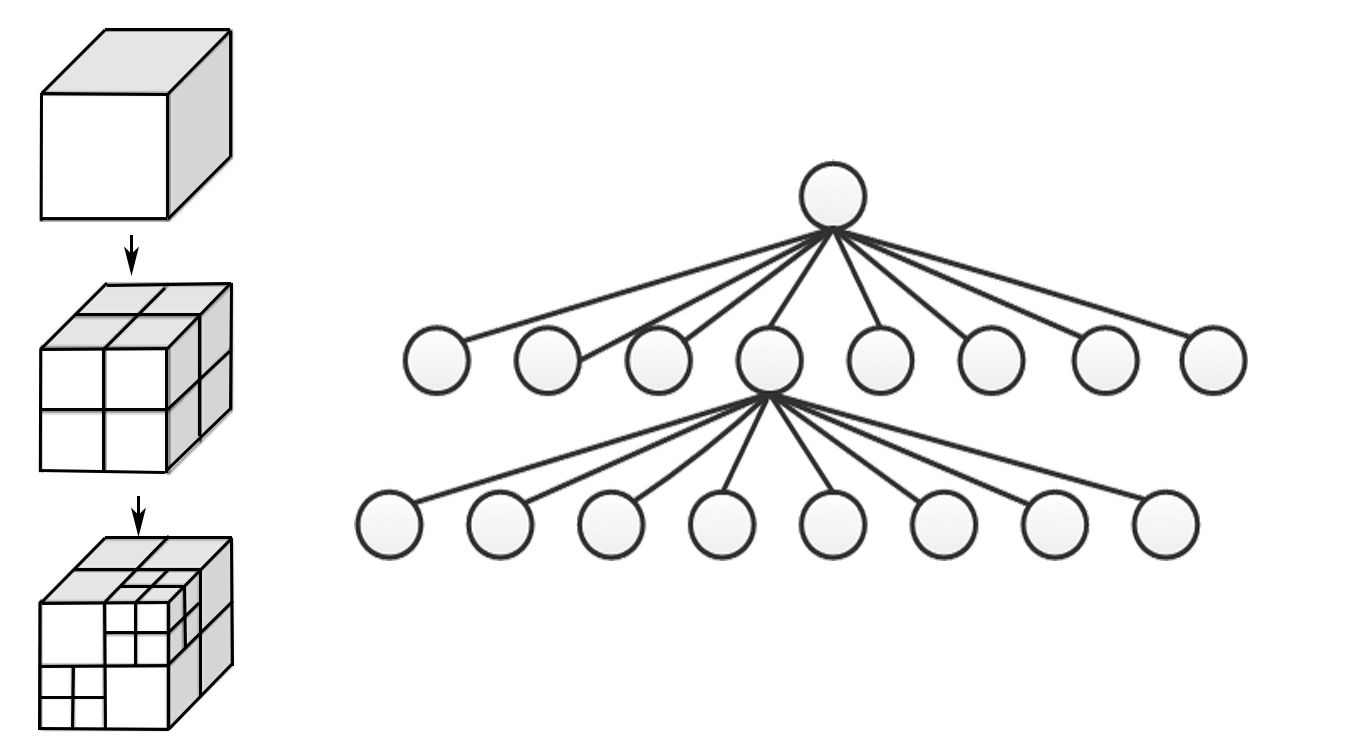
\includegraphics[width=0.75\textwidth]{Octrees.png}
	\caption{虚拟环境的八叉树划分}
	\label{fig:Octree}
\end{figure}
\par
如此划分得到的树是静态的和全局统一的。如果对于每一个立方体进行0~7的编号,整个虚拟环境中的每个大小立方体都可以用一组唯一的编号表示。通过将该序号编码在名称中,可以使名称表示特定的立方体。因此,对应名称的数据得到发布后,不论存储在哪个节点,该数据的含义是全局统一的。根据八叉树的划分结果,可以将每个节点的球形感知范围近似的用大小立方体表示。八叉树划分带来的主要优势是全局共享的命名空间:当节点A希望了解哪些对象在自己周围时,它可以分别根据A已知的存在于A的感知范围内立方体的立方体编号构成数据请求。如果没有统一的八叉树划分,A将使用自己位置和半径表达兴趣。如此,语义上讲,问题从谁在特定的区域中,变成了谁在给定(x, y, z)的R范围内。对于前者的问题,别的对同样区域感兴趣的节点可以共享该请求对应的应答;而对于后面的问题,由于短时间内另一个节点在完全相同的坐标发出完全相同的请求的概率很低,因此可以认为该问题的应答将只能对该请求者有效。况且,除了利用排除过滤的选择符(Exclusion filter),较难确保节点获取完整的问题答案。然而利用了排除过滤选择符后,往往会导致名称过长。综上,后者可以认为不是共享的命名空间,而八叉树划分提供了共享命名空间(Shared namespace),提高了数据共享的可能性。 
\subsection{发现模块}
\par
发现模块同样遵循局部性的设计要求。该要求可以诠释为,每个节点在任一时刻只希望了解自己的k-R最近邻居,该邻居由当前网络环境中唯一的节点名标识。相对于用固定的半径限制每个节点的感知范围,用kNN的优势在于其可以更好的利用网络资源。在节点所处的环境对象密集时,节点可以只获取最近的k个对象的位置,避免占用过大带宽。反之,在环境对象稀疏时,节点可以发现更远的对象。从游戏设计的角度来理解,可以视为是动态的调整感知范围的大小。
\par
发现模块利用八叉树划分的结果。每个节点了解自己所在的三维坐标,从而可以得到自己所在的立方体的编码,以及自己感知范围内包含的立方体的编码。对于处于自己感知范围内的立方体,节点通过名称注册接收和其相关的名称集合问题。同样由于前缀注册,对名称对应的立方体不了解或是不感兴趣的节点不会收到对应的数据请求。
\par
为了提高数据应答的利用率,同时确保收到的信息是完整的,本文在广播发现数据请求的名称最后添加了知识表达(Knowledge expression)字段。知识表达字段可以是对应立方体中本地了解的名称集的哈希。收到带有知识表达的数据请求的节点可以根据名称中包含的对象名称集的哈希值和本地已知的对象名称集的哈希值进行对比。仅当对于某一立方体,本地的对象名称集不同于收到的对象名称集时,收到数据请求的节点用自己集合内的对象名进行回答。
\par
综上所述,发现模块的命名空间可以用图\ref{fig:BroadcastNamespace}描述。
\begin{figure}[h!]
	\centering
	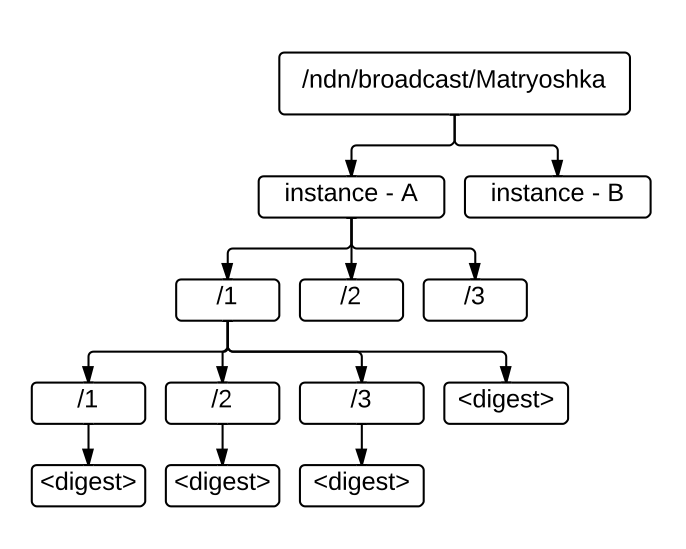
\includegraphics[width=0.70\textwidth]{DiscoveryNamespace.png}
	\caption{广播发现模块命名空间}
	\label{fig:BroadcastNamespace}
\end{figure}
\par
其中,最上层的时本应用的父命名空间;实体编号标识数据属于可能同时存在的多个实体中的哪一个(每一个对应一个独立的虚拟环境,不同实体中的游戏对象不需要发现对方);数字代表了八叉树立方体的编号;而digest代表了知识表达字段。
\par
收到的发现数据请求的数据应答应当由名称,所在的位置(最底层立方体)构成。由于没有任何一个节点是对名称中的立方体负责的,收到了名称并不代表本地对于该立方体的名称集合是不完整或是不正确的。在收到名称后,节点应当利用该名称构建对象位置的数据请求,从而真正确认是否本地的集合是不完整的。
\par
这样的哈希对应数据的表示方式体现了一个立方体的状态同步的步进过程,同时体现了将数据同步和状态同步分离的思想。相对于不把哈希值放在名称中的命名空间,这样的设计使得数据应答变得与数据存储位置无关。假设名称中没有哈希值,节点A在收到节点B关于立方体c的名称后,A没有办法确定B的答复是否准确。当A再次或是别的节点D同样表示对立方体c的请求后,如果请求经过了A、B间的缓存,获得的数据应答可能是B最初回复给A的不正确的,或是已经过时了的应答。
\par
然而上例体现了步进过程存在的一个问题。当一个节点的感知范围开始包括某一新的立方体时,该节点在获取到该立方体的最新信息前,可能会根据缓存中的内容给出的回复,对该立方体的历史状态进行遍历,直到获得最新状态。这样带来的问题是需要经过多个往返时间取得最新的状态。考虑到实时性的需求,本文利用ndnd-tlv支持的一项新选择符“必须为新鲜的“(Must be Fresh Child Selector)\footnote{参考在线文档,http://named-data.net/doc/ndn-tlv/interest.html}来减少获得过时信息的可能性。通过预设一个名称发现数据应答的新鲜时间,并且指定名称发现数据请求为”必须为新鲜的“,可以有效的通知缓存,本数据应答在多长时间内是有代表性的,在新鲜期过去后,该数据应答可以认为是过时的,不可以再次用来满足数据请求。
\par
根据上述逻辑,图\ref{fig:DesignSSD}展示了节点A通过节点B发现节点C的工作流程,在此给出作为发现模块的总结。
\begin{figure}[h!]
	\centering
	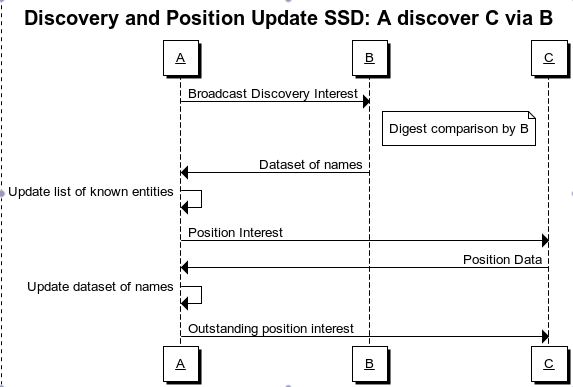
\includegraphics[width=0.70\textwidth]{SystemSSD.png}
	\caption{节点A通过B发现C的时序图}
	\label{fig:DesignSSD}
\end{figure}
\subsection{更新模块}
\par
每一个节点应当注册和自己的对象有关的数据请求前缀名称,即注册前缀包含自己的对象的名称的名称。
\par
发现模块将带来一系列的<对象名称-所在立方体编号>对。对于每一个名称,利用其构成位置数据请求(Position interest)和动作数据请求(Action interest),并向网络发送。利用之前所述的前缀注册过程,每一个的节点应当收到对自己位置的数据请求,对此该节点可以准确的作答。由于答案同样具有实时性的限制,在位置请求的数据应答中同样做以新鲜时间的设置,同时要求位置请求只获取新鲜的数据。
% Sample names
\par
综上所述,更新模块的命名空间如图\ref{fig:PositionUpdateNamespace}所示。
\begin{figure}[h!]
	\centering
	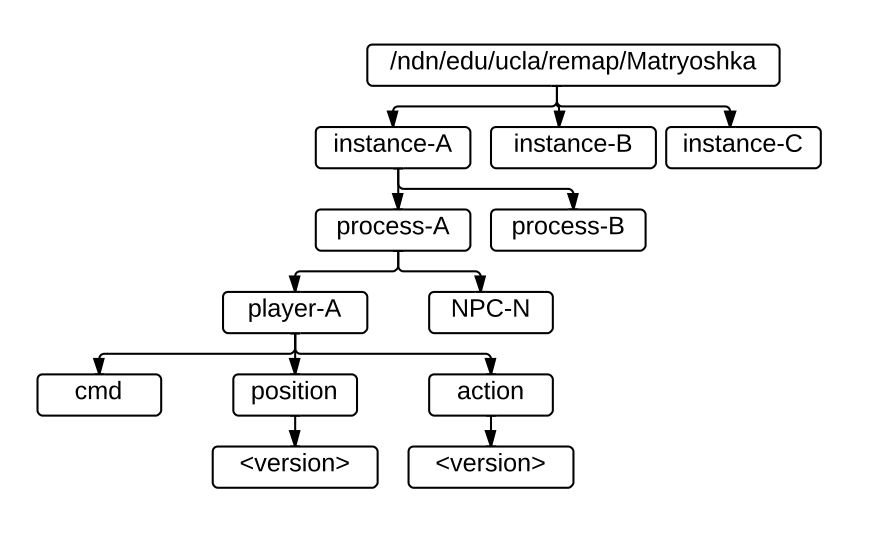
\includegraphics[width=0.90\textwidth]{PositionNamespace.png}
	\caption{更新模块命名空间}
	\label{fig:PositionUpdateNamespace}
\end{figure}
\par
为了确定是否需要对本地的立方体-名称集合表进行更新,更新模块应当记录每一个对象之前是否有被发现,以及其上一次被发现的位置在哪里。由于发现模块并不决定一个对象是否在其所述的立方体中,更新模块将根据几类不同的数据应答做出决定。
\par
收到了位置,位置属于自己感兴趣的立方体,位置所在的立方体和上次位置所在的立方体一致:应答节点在自己的兴趣范围内运动,本地应当渲染其现所在位置,并利用其现所在位置更新其上次位置。
\par
收到了位置,位置属于自己感兴趣的立方体,位置所在的立方体和上次位置所在的立方体不一致:应答节点从自己感兴趣的一个立方体进入了感兴趣的另一个立方体,本地应当渲染其现所在位置,并利用其现所在位置更新其上次位置,同时将其从之前的立方体的名称集合中移除,将其加入之后的立方体的名称集合。
\par
收到了位置,位置属于自己感兴趣的立方体,没有上次记录:新发现并确定应答节点存在,本地应当渲染其现所在位置,并利用其现所在位置设置其上次位置。
\par
收到了位置,位置不属于自己感兴趣的立方体,位置所在的立方体和上次位置所在的立方体不一致:应答节点离开了自己的感知范围,应当将其从上次的立方体的名称集合中删除,并不再渲染。同时把该节点从需要进行位置请求的节点名称列表中移除。
\par
收到了位置,位置不属于自己感兴趣的立方体,没有上次记录:收到了无关应答,可能由仍然处于预设的新鲜期内,但是实际已经过时的发现请求的应答导致。此情况下应该把该节点从需要进行位置请求的节点名称列表中移除。
\par
没收到位置,有上次记录:节点可能掉线,或是短时间无法应答。再次发出同样的数据请求。如果没有收到数据应答的次数达到预定阈值,则认为节点掉线,不再渲染,将其从上次位置对应的立方体的名称集合中删除。同时,把该节点从需要进行位置请求的节点名称列表中移除。
\par
没收到位置,没有上次记录:可能收到了错误、过时的节点名称,或是待被发现的节点暂时无法应答 。再次发出同样的数据请求。如果没有收到数据应答的次数达到预定阈值,则认为该节点不存在,把该节点从需要进行位置请求的节点名称列表中移除。
\section{面向对象设计}
\par
在完成了对交互过程和工作流程的描述后,本文从实现的角度描述设计方案具体包含的组件。本文采取的实现是面向对象的,图\ref{fig:DIscoveryModuleClassDiagram}为发现、更新模块项目实现的类图,由于篇幅限制没有展开。
\begin{figure}[h!]
	\centering
	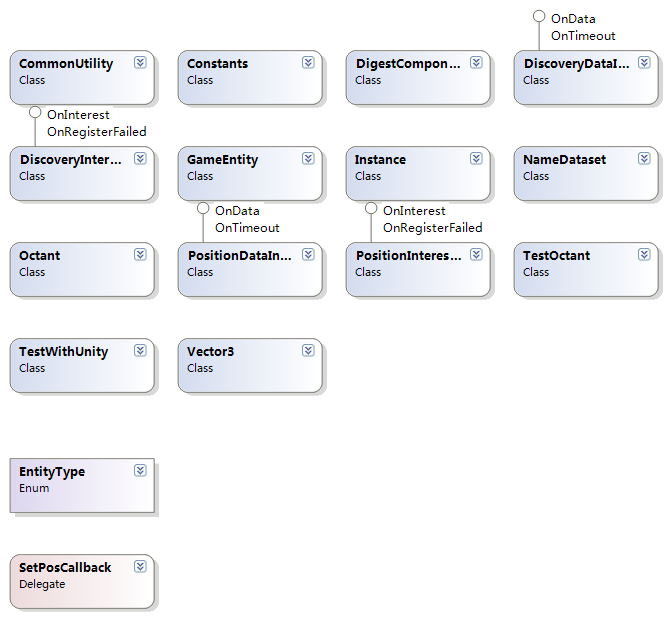
\includegraphics[width=0.70\textwidth]{DiscoveryModule.png}
	\caption{同步模块的类图描述}
	\label{fig:DIscoveryModuleClassDiagram}
\end{figure}
\par
其中主要类的功能介绍如下。
\begin{itemize}
\item
实体类(Instance):包含了请求、应答接口;存储本地的八叉树结构和每个树节点对应的哈希值和名称集;存储本地对象的相关信息和已知的对象列表;决定向哪个立方体和哪个对象发出数据请求;并在开始/结束时创建/终止线程实际进行发现/更新。
\item
发现请求接口类(DiscoveryInterestInterface):负责发现请求相关的请求处理。继承自OnInterest和OnRegisterFailed,重载请求处理函数。根据传入的Instance的引用对Instance中的本地八叉树结构中对应立方体的名称集和其哈希值进行访问并对收到请求做以应答。
\item
发现应答接口类(DiscoveryDataInterface):负责发现请求相关的应答处理。继承自OnData和OnTimeout,重载应答处理函数。根据传入的Instance的引用对Instance中的需要发出请求的对象列表进行书写。这里涉及到需要发出请求的对象列表的跨线程写入,因此需要互斥锁。
\item
更新请求接口类(PositionInterestInterface):负责位置请求相关的请求处理。继承自OnInterest和OnRegisterFailed,重载请求处理函数。根据传入的Instance的引用对Instance中的本地对象进行访问并对收到请求做以应答。
\item
更新应答接口类(PositionDataface):负责位置请求相关的应答处理。继承自OnData和OnTimeout,重载应答处理函数。根据传入的Instance的引用对Instance中的渲染对象列表进行书写。这里涉及到渲染对象列表的跨线程写入,因此需要互斥锁。
\item
八叉树节点类(Octree):负责八叉树节点及其名称集和哈希值的存储。本文中的树以左子右兄的结构存储。Instance中包含了此类型的八叉树根节点。
\item
游戏对象类(GameEntity):游戏对象类封装了游戏对象相关的属性,例如其名称、类型和位置,以及对游戏渲染函数等函数的回调入口。该类应当抽象出一个对象类,从而降低和游戏应用的耦合度。
\end{itemize}
\section{本章小结}
本章详细描述了命名空间,系统的设计逻辑。设计方案首先对虚拟环境进行统一的八叉树划分,形成共享命名空间,然后对划分得到的每个立方体进行同步。同步的过程为节点定时广播利用该立方体编号组成的名称以及名称集状态构成的发现数据请求。收到请求的节点返回名称集。发出请求的节点根据返回的名称组成含路由信息的位置请求,并利用该位置请求最终确定是否进行渲染,以及是否保持位置、动作的同步或作出怎样的更新。

% multiple1902 <multiple1902@gmail.com>
% intro.tex
% Copyright 2011~2012, multiple1902 (Weisi Dai)
% https://code.google.com/p/xjtuthesis/
% 
% It is strongly recommended that you read documentations located at
%   http://code.google.com/p/xjtuthesis/wiki/Landing?tm=6
% in advance of your compilation if you have not read them before.
%
% This work may be distributed and/or modified under the
% conditions of the LaTeX Project Public License, either version 1.3
% of this license or (at your option) any later version.
% The latest version of this license is in
%   http://www.latex-project.org/lppl.txt
% and version 1.3 or later is part of all distributions of LaTeX
% version 2005/12/01 or later.
%
% This work has the LPPL maintenance status `maintained'.
% 
% The Current Maintainer of this work is Weisi Dai.
%

\chapter{系统实现及测试}
\echapter{Implementation}
\label{ImplementationChapter}
\section{客户端函数库实现及测试}
\par
在描述了客户端函数库应当实现的功能和其类图结构之后,这里给出客户端函数库基于C\#语言的实现情况的概述。
语法上,Java和C\#是十分相似的。甚至有别的项目提供了Java到C\#语言的翻译工具(ref)。然而经过测试,翻译器的结果是不理想的。因此,作者基于Java函数库的语义,完成了C\#客户端函数库的实现。实现过程中需要注意的是两种语言提供的低层支持不同,例如Java.NIO中提供了可以用作缓存基础数据结构的高效字节缓存ByteBuffer类的实现;Java提供的传输层TCP网络接口与C\#提供的接口略有不同;Java应用RSA公钥算法加解密,附加、核实签名的方式不同于C\#;以及Java的异常抛出、处理机制和C\#不相同 。
\par
为了依然保持对上层的统一接口,作者及同事按照Java语言的文档在C\#语言中分别实现了上述不同之处。对应在源代码文件中,ByteBuffer的实现在ByteBuffer.cs中的net.named-data.jndn.ByteBuffer类;传输层接口的实现在TcpTransport.cs中的net.named-data.jndn.transport.TcpTransport类;Java的RSA私钥功能的辅助类的实现在net.named-data.jndn.security.certificate.PrivateKey类;异常处理机制体现在每个函数的throws部分的重写。
\par
函数库部分其它的实现与Java源码的逻辑近似,但是个别函数,例如获取当前的操作系统时间等采用了特定语言的调用。
客户端函数库附带了几个测试文件,用以测试函数库是否工作正常。TestEchoConsumer.cs实现Echo请求名称对应的数据应答;TestEncodeDecodeData测试用选择的编码格式编码、解码数据应答;TestEncodeDecodeForwardingEntry测试用选择的编码格式编码、解码数据请求的选择符;TestEncodeDecodeInterest测试用选择的编码格式编码、解码数据请求;TestGetAsync测试向指定的接口发送数据请求,是否可以得到预料的数据应答;TestPublishAsyncNdnx测试向本地的NDN daemon注册数据Echo请求前缀,并根据收到的Echo数据请求做以相应的数据应答。
\par
目前C\#客户端函数库的实现情况,除了从DER格式字节读入公钥、私钥外,已与5月31日的Java客户端函数库保持一致。 目前由于NDN daemon并不为各个应用发布它们应该使用的证书,而只要求可以利用数据应答的发布者提供的公钥能够核实数据应答的签名即可,所以C\#客户端函数库采用了一组提前预设的公钥私钥对,而不是从给定的DER格式字节读入。
\par
关于C\#客户端函数库的实现另外值得一提的一点是,作者原本尝试了利用IKVM工具,将Java源码编译对象指定为DotNet Assembly;或是利用IronPython将Python源码编译对象指定为DotNet Assembly,但是两个方案都行不通。前者的问题在于编译成的DotNet Assembly需要基于IKVM提供的DotNet Assembly,而后者包含Unity3D引擎不支持的DotNet基础库。后者的问题在于Unity3D支持的C\#语言版本过低,如果不利用C\# 4.0提供的dynamic关键字,IronPython编译结果会使得基本的函数调用代码很不工整。
\par
本部分的实现和简单说明可以在作者的Github站点\footnote{ndn-dot-net开发者函数库的作者Github链接,https://github.com/zhehaowang/ndn-dot-net}上找到。
\section{同步模块实现及测试}
\par
完成了同步模块功能的流程描述和类图描述后,本部分讲述同步模块的开发实现。同步模块实现采用的项目命名空间是remap.NDNMOG.DiscoveryModule,并包含子命名空间remap.NDNMOG.DiscoveryModule.Test。命名空间的命名满足C\#函数库命名空间命名的一般要求。设计部分描述的类均属于前一个命名空间。
\par
由于设计部分的功能描述已较为明确,实现时需要关注的重点有哈希函数、编码方式的选择,参数的选择,和对上层提供的接口。
\subsection{哈希函数、编码方式和参数选择}
\setcounter{subsubsection}{0}
\par
由于本文涉及的名称字符串数量不多,长度较少,本文首先对所有字符串做以异或,得到一个字符串后采用FNV哈希计算Digest值。哈希函数的实现继承自只包含功能的父类,因此哈希函数可以较为轻松的修改。
\par
在选择完哈希函数后,需要对得到的整型做以向URI的转换。本文采用了Base64的编码方式,将整型二进制直接编码为字符串。Base64不足的部分采取补0。在优化中提到的\ref{MultiLevelOptimizationSection}部分后,编码的格式如下。
\newline
\centerline{<type - relative octant index - digest - relative octant index 2 - digest 2>}
\par
本应用涉及到的主要参数有。
\subsubsection{32位FNV哈希常量}
大质数值设置为16777619;偏移量值为2166136261;
\subsubsection{超时时间和间隔时间常量}
发现请求的超时时间为10秒,发现请求的最小间隔为3秒,应答的新鲜时间为20秒;位置请求的超时时间为0.5秒,位置请求的最小间隔为0.25秒,应答的新鲜时间为1秒;
\subsubsection{八叉树层数及可以注册请求前缀的有效层数}
八叉树对虚拟环境的默认划分层数为7层,从第5层开始可以注册前缀;
\subsubsection{掉线判定的超时位置请求个数}
连续收到20个位置请求超时将认为节点掉线。
\par
经测试,以上参数的选取在网络广播流量上和更新速度上,即从实时性和大规模可拓展性的要求上而言是比较合适的。
\par
最后描述一点实现过程中为了降低和游戏应用的耦合度所做的优化。由于同步模块是独立的DotNet Assembly(mono dll),其应该被游戏应用调用。游戏应用应向其提供本地对象的位置,并读出同步模块提供的周围其它对象的位置及行动,从而进行渲染。为了减少二者间的耦合度,同步模块的用例类可以接收调用者传入的一个回调函数。因此,在游戏应用中实例化用例类时,将渲染入口传入,即可以利用同步模块的工作结果进行周围其它对象的渲染。
\par
本部分的实现和简单说明可以在作者的Github站点\footnote{同步模块的作者Github链接,https://github.com/zhehaowang/DiscoveryModule}上找到。
\subsection{测试}
\par
同步模块的测试分为2个部分。模块本身包含了测试文件,用以模拟产生一个用例类,并进行发现,同时输出八叉树的情况和Base64编码的哈希值,以观察模块基本功能是否工作正常。模块还在多台机器运行的实际的游戏应用中进行了测试。实际测试的环境如下。
为两个运行Mac OSX 10.8和10.7的计算机,分别生成游戏二进制文件,通过配置文件为生成的二进制文件赋予用于发布位置、行动等信息的用例名。在两台计算机上配置并运行ndnd-tlv。
\par
这里由于篇幅的限制,作者不讨论ndnx或是ndnd-tlv的安装、配置过程;其与ndn-cpp函数库,ndn-cxx函数库的关系;以及其与ccnd、ndnd和NFD的兼容性问题。该过程中可能遇到的问题在项目对应的redmine站点\footnote{安装配置ndnd-tlv的相关信息链接,redmine.named-data.net/projects/ndnd-tlv/wiki},或是作者的github代码工程的readme中可以找到。
\par
之后为二者都添加到一个NDN公用节点aleph.ndn.ucla.edu的TCP连接。这里应当注意要使用该节点提供的可创建路由回路的前缀列表中的前缀,从而使得多个节点互相发送的发现数据请求可以被该节点正常前递到应该收到请求的节点。添加连接的命令类似ndndc add /ndn/edu/ucla/remap tcp aleph.ndn.ucla.edu,其中/ndn/edu/ucla/remap是aleph提前配置好可以供本应用注册的名称前缀。
\par
经测试,在三台计算机上进行同样的操作,并同时运行六个游戏实体时,多台计算机上运行不同的游戏应用互相发现对方,并获得对应的位置更新。但是可以更经常的观察到位置更新并不及时。在上述配置和运行环境下,位置的更新基本为1秒钟3次。运行游戏节点的平均吞吐量为0.6KB/s。1秒3次的更新并无法满足要求,其限制因素主要在于当前NDN路由进程位置应答的新鲜时间最少为1秒,因而应用需要使用版本信息对位置进行过滤,该功能当前还在实现中。
\par
测试所用的单元测试文件包含在对应的功能模块的Github库中;游戏测试文件可以在作者的Github库\footnote{游戏应用的Github链接,https://github.com/zhehaowang/NDNMOG-live}中找到。
\par
在完成了上述的基本实现后,本文对设计方案做出了诸多优化,具体在\ref{OptimizationSection}部分一一叙述。
\section{本章小结}
本章提供了本应用涵盖的三层,即开发者函数库层,同步模块层和游戏应用层的实现细节和初步的测试结果。实现细节并没有具体到每个类实现的功能和实现时作出的选择。细节性的内容可以在每层对应的Github链接中看到代码和说明。
% multiple1902 <multiple1902@gmail.com>
% intro.tex
% Copyright 2011~2012, multiple1902 (Weisi Dai)
% https://code.google.com/p/xjtuthesis/
% 
% It is strongly recommended that you read documentations located at
%   http://code.google.com/p/xjtuthesis/wiki/Landing?tm=6
% in advance of your compilation if you have not read them before.
%
% This work may be distributed and/or modified under the
% conditions of the LaTeX Project Public License, either version 1.3
% of this license or (at your option) any later version.
% The latest version of this license is in
%   http://www.latex-project.org/lppl.txt
% and version 1.3 or later is part of all distributions of LaTeX
% version 2005/12/01 or later.
%
% This work has the LPPL maintenance status `maintained'.
% 
% The Current Maintainer of this work is Weisi Dai.
%

\chapter{系统分析、评估及优化}
\echapter{Evaluation}
\label{EvaluationChapter}
\section{系统分析}
\par
本部分首先给出系统的简单测试结果,然后给出系统的理论分析结果。
\par
由于当前运行的NDN节点数量较少,可用的硬件设施也不多,基本不具备大规模实际测试的条件,本项目进行的测试仍然是少量节点运行多个游戏实例,并度量本地节点发出移动命令,至远程节点接收移动信息更新的时间差。
\par
在进行简单实际测试之后,本文根据需求分析部分提供的几点要求,理论的对系统做出分析和评估。
\begin{itemize}
\item
局部性

八叉树划分,并且只对自己感兴趣的立方体进行同步体现了局部性的要求。如此发出数据请求和注册名称前缀会使得发出数据请求的节点不发出多余的信息,而接收到数据请求的节点收到的内容逻辑上也都和自己相关。
\item
实时性

本文的设计方案从两方面满足实时性的要求。一方面由于命名空间是共享的,通过合理的八叉树大小的配置,广播发现数据请求可能被多个节点共享的可能性较大。另一方面,每个数据请求只获取新鲜数据,并且每个数据应答有相应的新鲜周期,所以更新过程不会受到过期数据的影响。
\item
大规模可拓展性

通过将状态同步和数据同步分离,将广播发现过程和位置、动作更新过程分离,本文的设计方案在理论上有较高的效率。而下面所述的系统优化将有助于可拓展性进一步提升。
\item
健壮性

这里分别讨论网络分块、发现数据请求乱序、丢包和位置数据请求乱序、丢包造成的影响。由于发现数据请求一直在被定时广播,出现网络分区后,一旦连通性恢复,节点间的互相发现不应该受到影响。同时,发现数据请求的应答出现丢包或是乱序对系统没有严重影响。对于丢包的情况,请求发送方会收到请求超时并重新发送发现请求;对于乱序的情况,位置应答而不是发现应答对渲染哪些对象有决定权,所以也不会对系统有影响。位置数据请求如果丢包,会导致请求方短时无法更新对象的位置;而位置数据请求会包含本地时间的时间戳,如果出现乱序,时间戳靠后的位置被渲染后收到时间戳考前的位置,后者不会被渲染。
\end{itemize}
\par
综上,系统对网络可能出现的异常有一定抵抗力。
\section{系统优化}
\label{OptimizationSection}
\par
本部分记述已经实际应用于项目实现中的优化。
\subsection*{多个数据请求合一}
\label{MultiLevelOptimizationSection}
\par
考虑图中用例,如果对于每个立方体分别发出数据请求,数据请求的数量会较多。
\par
利用八叉树划分虚拟环境的优势之一是利用八叉树的层次结构,即不止对叶子节点发出发现数据请求。在数据请求的发出方了解到自己的数据请求可以利用八叉树结构进行合并时,数据请求的发出方会对最后的哈希字段做以重新的编码。对于上图中的用例,需要发出的数据请求发生了如下变化。
\par
如此优化带来的好处有大大减少发出的数据请求数量,和注册的前缀数量。原本的思路中,每个大小立方体对应一个独立数据请求和注册前缀。现在,注册的前缀只用包括几个包含感知范围的立方体的特定层的父节点;而发出的数据请求的数量会动态的发生变化,其变化与之后的渐进性发现的优化思路有关。另外,这样的优化更加自然,因为其利用了八叉树本身提供的树形结构,而不是将其等同于一维编码,例如基于康拓配对或希尔伯特曲线的划分。
\par
\subsection*{渐进性发现}
\par
渐进性发现的含义有两点。允许收到数据请求的节点在不具有完整的被请求信息时进行回复;以及允许每个节点动态的调整自己的感知范围大小。
\par
第一点的问题来自于上一则优化。
\par
由于数据请求的合一,节点收到的数据请求包含的区域不一定和本地拥有的或感兴趣的信息完全吻合,从而为节点做出应答带来了困难。
\par
当数据请求包含的区域是本地感兴趣的区域的子集时,节点可以通过解码、匹配到对应区域并作答;
\par
当数据请求包含的区域与本地感兴趣的区域完全不相交时,节点不予作答并在预设时间过去后请求超时;
\par
而考虑二者的中间情况,即当数据请求包含的区域与本地感兴趣的区域部分相交,换言之,本地感兴趣的区域包括数据请求包含区域的子集。节点如果作答,可能导致请求者收到不完整的答案,请求者需要根据不完整的答案重新核实,并修正自己的哈希值字段,然后重新发布发现数据请求,并且希望这次的哈希值同有着不完整信息的节点的哈希值相同,从而其不会作答。在此期间,有完整数据的节点可能也会收到数据请求 ,并试图作答,但是为了保证收发平衡,其答案会由于重复而被路由节点丢弃。最终导致的结果是数据请求节点为了获得完整的信息,反而付出了更长的时间。节点如果不作答,则对于接收节点而言,自己接收了没有意义的信息;对于发送节点而言,相当于其要求网络中的接收节点拥有的区域与自己发出的请求代表的区域完全吻合,这样的情况可能较少出现。对此,本文提出了一个折中方案。接收节点可以作答,但是其会主动延迟应答发出的时间。延迟时间和二者区域的重合程度成反比,即区域的交集占数据请求中区域的比例越大,延迟的时间越少。而最初叙述的两种简单情况也可以视为二者的比例为1时,接收请求的节点立刻作答;二者的比例为0时,接收节点推迟无穷大时间。
\par
在解决了这一问题后,渐进性发现还有一点含义,即允许节点根据当前所在虚拟环境的密集程度和网络是否拥塞动态的调整自己的感知范围。这一点即为kNN问题的实际用例。数据请求指向的立方体不再由固定的感知范围定义,而由节点根据自己了解到的周围对象数量的多少步进式的动态调整。
\par
例如,节点首先试图获取R范围内包含的立方体中的对象,如果对象数量未达到k个,则R自增一个单位,直到对象数量满足要求。对于收到的所有对象名称,节点根据其位置进行排序,并且只渲染其中最近的k个。这里R自增一个单位的方式可以利用kd树的kNN查找,由于在\ref{kNNIntroSection}部分已经有所介绍,这里不再赘述。另外一种自增的方式是实际考虑本地对象当前的速度和朝向,并且加入该朝向上的一个叶子立方体。后者的实现可能会不太稳定。
\par
\subsection*{事件驱动为主的请求发送}
\par
在上述的设计思路中,发现数据请求是定期广播的。为了保证发现的及时性,广播的周期不能很长,而为了减少流量,广播的周期也不能过短。本部分引入事件驱动为主的请求发送,从而进一步减少广播发布的数据请求数量。简而言之,每当本地对象新启动游戏,移动或渐进性发现导致了感知范围包含新的立方体时,节点对该立方体以较高的频率发布广播发现数据请求。其它情况下,节点对该立方体以较低的频率发布广播发现数据请求。这样做设计上较为自然,即在已知区域基本达到稳态后,各个节点基本不需要再通过广播发现数据请求维持状态上的同步从而了解对象的去留,而仅通过单播的对象位置信息,就可以清楚对象的去留。而当节点对新的立方体产生兴趣时,无论是因为节点加入、感知范围扩大还是本地对象移动,节点应当积极的获取新立方体中的状态并与其同步。在这一过程中并不可以完全摒弃低频率的广播数据请求发送。一方面在特定的网络连接下,广播数据请求可以促进新的节点加入且其名称被一个感兴趣的节点发现后,更早的被别的感兴趣的节点发现;另一方面,广播数据请求可以使得游戏从一些网络异常现象中恢复,比如网络分块。
\section{其它设计思路及对比}
\label{ComparisonSection}
\par
分析和评估的重点内容是和其它设计思路的对比。本部分记述设计过程中作者所主要考虑的其它设计思路,并和其一一做以对比。下面叙述的几个设计思路分为两大种类,第一种是基于NDN网络的,由作者在项目初期提出,经过理论分析后,作者认为无法很好的描述项目的需求;第二种是基于IP网络的,由别的研究人员在过去的10年中提出,与这些方案的对比较难进行,因为NDN网络还处于试验阶段,且我们缺乏的硬件条件和测试标准使得实际的测试有说服力。
\subsection*{基于位置敏感哈希的划分}
\par
LSH方法的原理在背景部分已经有所介绍。基于LSH的方案不同于本文所提的方案,主要在于不再采用八叉树对虚拟空间进行划分,而采用两组预定的p稳定的哈希函数对虚拟空间进行划分。这里依然把LSH视为划分,是为了更直接的体现共享命名空间的概念。划分之后的步骤同本文重点描述的方案相近,但是可以更好的利用如\cite{LSHKNNRef}中描述的基于LSH的kNN算法。
\par
对于一个输入坐标(x, y, z),第一组k个哈希函数得到一个k维向量,对于该k维向量,第二组哈希函数得到一个值,即为该坐标所属于的虚拟分区桶编号。在第一步中使用多个函数的原因是用多组相交的平面可以更好的划分出虚拟空间对应的形状,并用其模拟球形的感知范围。采取这样的划分的原本目的亦是如此,即通过多个哈希函数的限制反映球形的感知范围,如图即为二维输入下圆形感知范围的模仿。
\par
然而在实际测试中,LSH的效果并不良好。问题在于步骤二。如果认为桶的数量足够多,不考虑取模对值的影响,在应用了第二组哈希函数后,整个过程的效果变为在第一步中仅运用一个哈希函数,即用两个平行的平面对虚拟空间进行划分。
除此之外,LSH本身并不适合三维,或是综合考虑时间后,四维的用例。因为,第一组哈希函数的应用可以认为是在丢失一定量信息的高维到低维的维度缩减,而为了保证高维下的距离相对关系在维度缩减后仍有较高的概率保持不变,第一组函数往往需要选取多于4个。对于我们的用例,输入量本身的维度很低,维度减少并不是需要考虑的核心问题。
\par
综上所述,再加上LSH方法不能很好的应用多层的划分(如果直接采用值大小的多层划分,LSH依然存在边界问题,即不能很好的解决最初提出时希望解决的球形划分的问题),我们认为基于LSH划分的思路不会在表现上优于本文主要描述的方案。本文所用的LSH测试方案可以在作者的Github站点找到\footnote{作者的LSH相关的测试,https://github.com/zhehaowang/PStableLSHC,\newline以及https://github.com/zhehaowang/PStableLSHCSharp}。
\subsection*{基于可逆转Bloom Filter的知识表达}
\label{IBFComparisonSection}
\par
可逆转的Bloom Filter(Invertible Bloom Filter, IBF)的原理在\ref{IBFIntroSection}部分已经有所介绍。基于IBF的设计方案的提出原本是为了用立方体的对象名称集的IBF取代哈希值的知识表达字段,即发现数据请求名称中的最后一个组成部分。
\par
使用IBF的优势在于可以直接编码对象名称,在两个名称集的不同的元素数量较少的情况下,接收方有较高的概率可以直接解码出对象名称。因此,相对于文中重点描述的方案,基于IBF的方案在获取到数据请求的发送者拥有哪些名称上可以少一个数据应答的时间。另外,考虑到IBF的表现在两个名称集的交集较大,而差集很小的情况下较为出色,而名称集的同步从一个稳态过渡到另一个稳态的过程恰巧符合这个特点,IBF显得更加适合我们的用例。
\par
然而,IBF具有以下的缺点。首先,差集的恢复是概率性的,为了提高恢复的概率,IBF的大小必须提高,即拥有更多的哈希桶。这意味着广播数据请求的长度也会相应提高。由于广播数据请求会更多的被发送,其长度应该尽可能的被减小,而为了从10个名称中拥有90\%的概率恢复出3个不同的名称,IBF会为数据请求名称增加200个字节,这在作者认为是不值得的。其次,IBF无法很好的利用八叉树的层次结构。如果\ref{OptimizationSection}部分中头两点方案,除了广播发现数据请求的名称会变得过长外,在节点接收到的发现数据请求描述的区域和自己了解的区域不完全相同时,IBF会退化为普通BF,意味着其可能漏过不同的名称。
\par
综上考虑,本文并没有最终使用基于IBF的设计方案。作者为测试用而实现的IBF结构可以在作者参与合作的Github站点找到\footnote{基于IBF和CCNx实现的游戏应用代码链接,https://github.com/CherryQu921/NDNMOG/tree/npc}。
\subsection*{部分P2P思路}
\label{PartialP2PSection}
\par
部分P2P的思路的核心在于动态的选择某个节点,使其为某一个区域负责,即掌管该区域的名称集,并通知其它节点自己为该区域的负责人。由此,对该区域感兴趣的节点问网络的问题变成了谁是区域的负责人,而在拥有了负责人名称之后,节点的问题变为向负责人询问它的名称集,或是通知负责人自己的加入或是离开。如此,为了实现各个区域的同步,所有对该区域感兴趣的节点只用不断的请求负责节点的名称集即可。而在负责人离开后,其需要指定下一任负责人,或是通知各个感兴趣的节点进行选举,并将信息移交给下一任负责人。
\par
部分P2P是IP的P2P游戏联机的主要思路之一。其显著的优点在于除了负责人替换的策略外,控制相对简单,且完成同步所需的网络流量也可能会相对较小。
\par
本文并没有重点探究部分P2P的思路,一方面是因为负责人替换策略比上面描述的要复杂许多,因为要考虑负责人非正常离线等情况导致的信息无法正常交接,和负责人协商的过程本身也需要多个节点的同步和解决冲突。另一方面是因为我们的用例作为NDN多人联机游戏,数据存储的位置的重要性应该得到弱化,因此不希望采取一个依然拥有逻辑上的小规模“服务器”的策略。
\par
在这两种架构的选择背后有更深层的研究和讨论,目前并没有一种优于另一种的定量结论,二者的区别更多地是被看做设计理念上的不同。而本文描述的应用也可以看做是主观上希望尽可能的探究纯P2P结构的大型网络联机游戏的可能性。
\subsection*{IP网络下的P2P实现}
\par
IP网络下有许多P2P多人联机游戏的实现方案。最为流行的思路是基于DHT中间层的。大体而言,是通过建立和维护一张将虚拟环境游戏状态映射到为该游戏状态负责的节点的IP地址或是到达该节点的下一跳IP地址的分布式哈希表,解决IP网络自组织多人联机游戏的核心问题:从哪里获取数据。在DHT的部署上或是哈希的内容上,不同文章的做法不尽相同。Pastry系统\cite{IPP2PMMORPG1}的思路是将参与游戏的所有节点和所有游戏对象的ID进行哈希;而\xjtuincite{IPP2PMMORPG2}先将虚拟环境进行划分,为每个分区动态的选择负责人,并将分区和负责人信息进行哈希,更加类似基于多播的Pub/Sub系统\cite{PubSubRef}。
\par
在这些思路中,DHT的存在体现了IP网络中“地址”扮演的重要性,同时也体现了,在拥有一个物理环境主持一个虚拟环境,二者不存在直接的映射;且就希望优化的量而言,传输效率是对物理环境的要求,而局部性是对虚拟环境的要求,的情况下,IP对物理环境或物理位置的过度强调,使得应用的设计并不自然。本文的NDN游戏应用将考虑的核心放在了“问网络怎样的问题”上,而不是“从哪里获取答案”上,更加贴近了应用层的开发理念,省去了不自然的DHT中间层,也利用了NDN网络对多播的天然支持,争取得到效率上最大化的提升。
\subsection*{IP网络下的C/S实现}
\par
传统MMORPG是基于客户端/服务器结构实现的。服务器将为游戏状态及用户账户负责。C/S架构下的可拓展性是通过服务器集群实现的。多台服务器间可以通过局域网相连,比如Terazona\footnote{简单介绍,http://www.businesswire.com/news/home/20030303005397/en/Zona-Announces-Terazona-Network-Engine-Support-Capcom\#.U5pKKY0Ybb4}中描述的;或是组成计算网格,如Butterfly.net中\footnote{参考书籍,Official Butterfly.Net Game Developer's Guide}描述的。尽管这种架构通过增加服务器的数量,优化服务器的策略可以使得更多的玩家同时享受服务,它仍缺少自组织网络的灵活性,并且就目前的实施情况来看,服务器总是无法很好的应对服务需求的高峰期。同时,C/S架构的游戏限制了当今游戏的另一个发展趋势,用户开发游戏的部署。尽管像EverQuest等的游戏允许用户自主设计游戏扩展,然而安全和效率的问题仍然会限制这些拓展的数量和体积,因为他们都需要在为游戏状态负责的服务器上统一存在。
\par
尽管C/S架构存在许多潜在的问题,目前商业化的网络游戏仍然没有采用P2P架构的。目前P2P架构相对于C/S架构的优点更多只有于定性的理论分析。如\ref{PartialP2PSection}所述,二者是设计理念上的不同。而基于新网络架构的P2P实现可能会为两种架构的讨论带来新的思路,机遇和挑战。
\section{本章小结}
本章对系统是否达到了需求中的要求进行了理论分析。在此之上,本章对系统提出了三点优化方案,目前三点方案已经实现,但是还没有进行系统的测试。最后,本章将本文的设计方案和我们早期的三种思路,和IP下的两种思路进行了对比。

% multiple1902 <multiple1902@gmail.com>
% conclusion.tex
% Copyright 2011~2012, multiple1902 (Weisi Dai)
% https://code.google.com/p/xjtuthesis/
% 
% It is strongly recommended that you read documentations located at
%   http://code.google.com/p/xjtuthesis/wiki/Landing?tm=6
% in advance of your compilation if you have not read them before.
%
% This work may be distributed and/or modified under the
% conditions of the LaTeX Project Public License, either version 1.3
% of this license or (at your option) any later version.
% The latest version of this license is in
%   http://www.latex-project.org/lppl.txt
% and version 1.3 or later is part of all distributions of LaTeX
% version 2005/12/01 or later.
%
% This work has the LPPL maintenance status `maintained'.
% 
% The Current Maintainer of this work is Weisi Dai.
%
\chapter{结论与展望}
\echapter{Conclusion}
\label{ConclusionChapter}
\section{结论}
\par
NDN是一种以数据及其名称为基本对象的新网络架构。本文提出、测试并理论分析了一个在NDN网络中运行的纯P2P的多人联机游戏应用的设计方案。该方案面临的主要问题是在分布环境下各个节点信息的同步,即每个节点需要通过和网络交互,获取谁在我的周围,以及它在哪里,在做什么等问题的答案。
\par
方案首先对虚拟环境进行固定的八叉树划分,并对划分后得到的每个小立方体中的对象的名称集进行同步。各个节点定时广播本地感知范围内的立方体的名称集的消息摘要,收到不同的消息摘要的节点回复本地的名称集。收到包含不同名称的数据应答的节点根据其中的名称构成位置和动作数据请求,从而获得具体节点的位置,并决定是否渲染,以及是否加入到本地对应立方体的名称集中。
\par
方案满足了局部性、实时性、可拓展性和健壮性的要求。在详细叙述方案后,本文分析了实际测试的结果,并详细分析了和早期的三个设计方案,和IP下的实现的优劣的对比。
\section{展望}
\par
本文涉及到的工作在许多方面仍然有可以改进之处。
\par
进行实际环境的测试和IP下不同实现的对比。构建类似功能和参数的IP下的C/S和P2P架构的实现,并衡量每个节点的出入流量,延迟时间,从而得到在更大规模的环境下本方案是否可行,和IP相比优劣如何的结论。
\par
测试优化中提出的数个思路是否对效率的提升起到作用。并为位置数据应答设计和实现版本信息,在数据请求中过滤版本信息,从而获得更多更为连贯的最新位置更新。
\par
游戏渲染优化。插值和预估是使渲染流畅的常用策略。插值使位置渲染平滑化;预估使得一个往返时间的延迟固定存在时,延迟看起来更小。



\xjtuendcontent

\xjtubib{bibliography.bib}

\xjtuappendix
% multiple1902 <multiple1902@gmail.com>
% appendice.tex
% Copyright 2011~2012, multiple1902 (Weisi Dai)
% https://code.google.com/p/xjtuthesis/
% 
% It is strongly recommended that you read documentations located at
%   http://code.google.com/p/xjtuthesis/wiki/Landing?tm=6
% in advance of your compilation if you have not read them before.
%
% This work may be distributed and/or modified under the
% conditions of the LaTeX Project Public License, either version 1.3
% of this license or (at your option) any later version.
% The latest version of this license is in
%   http://www.latex-project.org/lppl.txt
% and version 1.3 or later is part of all distributions of LaTeX
% version 2005/12/01 or later.
%
% This work has the LPPL maintenance status `maintained'.
% 
% The Current Maintainer of this work is Weisi Dai.
%
\xjtuappendixchapter{附录}

    \xjtuappendixsection{测试标题}

        The quick brown fox jumps over the lazy dog.

        \begin{figure}[h!]
          \centering
          
\includegraphics[width=6.67cm]{XJTU.pdf}
          \caption{西安交通大学}
          \label{fig:in-appendix}
        \end{figure}

        \xjtuappendixsubsection{三级标题}

            测试

            \xjtuappendixsubsubsection{四级标题}

                测试

\xjtuappendixchapter{还是附录}

    \xjtuappendixsection{测试}

        The quick brown fox jumps over the lazy dog.

\xjtuendappendix

\xjtuspchapter{致谢}{致\qquad 谢}
\par
首先感谢我的指导老师,西安交通大学的安健老师,美国加州大学洛杉矶分校的Prof. Jeff Burke和Prof. Lixia Zhang的耐心指导。
\par
感谢西安交通大学和加州大学洛杉矶分校为我提供的机会。
\par
感谢父母对我的支持。
\par
感谢电信硕01班班主任朱正东老师、刘纯亮老师和各位同学对我的帮助。
\par
感谢Xingyu,Zening,Jeff. T,Alex,Anmol,Daisuke,Cole,Zoe等UCLA的同事、同学对我工作的兴趣,提供的支持和帮助。
\par
感谢Panasonic的Muramoto先生和西北大学的Xiaojiang Chen教授对我工作表示的浓厚兴趣。
\par
感谢XJTUThesis项目,特别感谢戴唯思同学提供\LaTeX模板。

\end{document}

